
\chapter{The Top Level Structure of the Proof}

%\section{Overview}
\label{sec:overview}

This \chap\ describes the structure of the proof of the
\index{Kepler conjecture} Kepler conjecture.
%\footnote{This research is supported in part by the NSF.} % MOVED TO END OF PAPER.

\section{Statement of Theorems}\label{sec:statement}


\begin{theorem}[The Kepler Conjecture]
\label{theorem:kepler}   No packing of congruent balls in
Euclidean three space has density greater than that of the
face-centered cubic packing.
\end{theorem}

This density is $\pi/\sqrt{18}\approx 0.74.$

\begin{figure}[htb]
  \centering
  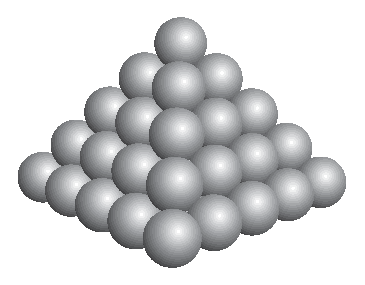
\includegraphics{PS/fcc_small.eps}
  \caption{The face-centered cubic packing}
  \label{fig:fcc}
\end{figure}


The proof of this result is presented in this paper. Here, we
describe the top-level outline of the proof and give references to
the sources of the details of the proof.

\shortversion{An expository account of the proof is contained in
\cite{CH}.  A general reference on sphere packings is \cite{CS}.  A
general discussion of the computer algorithms that are used in the
proof can be found in \cite{algorithm}.  Some speculations on the
structure of a second-generation proof can be found in
\cite{arbeitstagung}. Details of computer calculations can be found
on the internet at \cite{web}.}

\shortversion{The current paper presents an abridged form of the
proof.  The full proof appears in \cite{KC}. Samuel P.
Ferguson\index{Ferguson} has made important contributions to this
proof.  His University of Michigan thesis gives the proof of a
difficult part of the proof \cite{thesis}.  A key \chap\
(\Chap~\ref{sec:scoring}) of this paper is coauthored with
Ferguson.\index{Ferguson}}


By a {\it packing}, we mean an arrangement of congruent balls that
are nonoverlapping in the sense that the interiors of the balls are
pairwise disjoint. Consider a \index{packing} packing of congruent
balls in Euclidean three space. There is no harm in assuming that
all the balls have unit radius. The density of a packing does not
decrease when balls are added to the packing. Thus, to answer a
question about the greatest possible density we may add
nonoverlapping balls until there is no room to add further balls.
Such a packing will be said to be {\it saturated}.
%
 \index{saturated}
 \index{overlap}

Let $\Lambda$ be the set of centers of the balls in a
\index{saturated} saturated packing. Our choice of radius for the
balls implies that any two points in $\Lambda$ have distance at
least $2$ from each other. We call the points of $\Lambda$ {\it
\index{vertex} vertices}.  Let $B(x,r)$ denote the closed ball in
Euclidean three space at center $x$ and radius $r$. Let
$\delta(x,r,\Lambda)$ be the finite density, defined as the ratio
of the volume of $B(x,r,\Lambda)$ to the volume of $B(x,r)$, where
$B(x,r,\Lambda)$ is defined as the intersection with $B(x,r)$ of
the union of all balls in the packing. Set $\Lambda(x,r) = \Lambda
\cap B(x,r)$.\index{ZZdelta@$\delta(x,r,\Lambda)$}

Recall that the \index{Voronoi cell} Voronoi cell
$\Omega(v)=\Omega(v,\Lambda)$\index{ZZzomega@$\Omega(v)$} around a
vertex $v\in \Lambda$ is the set of points closer to $v$ than to
any other ball center. The volume of each Voronoi cell in the
face-centered cubic packing is $\sqrt{32}$.  This is also the
volume of each Voronoi cell in the hexagonal-close packing.

\begin{definition}\label{def:negligible}
Let $A:\Lambda\to\R$ be a function.  We say that $A$\index{Az@$A$}
is
  {\it negligible\/}\index{negligible}
if there is a constant $C_1$ such that for all $r\ge1$ and all
$x\in\ring{R}^3$, we have
   $$\sum_{v\in\Lambda(x,r)} A(v) \le C_1 r^2.$$
We say that the function $A:\Lambda\to\R$ is
  {\it fcc-compatible\/}\index{fcc-compatible}
if for all $v\in\Lambda$ we have the inequality
$$\sqrt{32}\le \op{vol}(\Omega(v)) + A(v).$$
\end{definition}

The value $\op{vol}(\Omega(v)) + A(v)$ may be interpreted as a
{\it corrected\/} volume\index{corrected volume} of the Voronoi
cell. Fcc-compatibility asserts that the corrected volume of the
Voronoi cell is always at least the volume of the Voronoi cells in
the face-centered cubic and hexagonal-close packings.




\begin{lemma}
\label{lemma:deltabound} If there exists a \index{negligible}
negligible \index{fcc-compatible} fcc-compatible function
$A:\Lambda\to\R$ for a saturated packing $\Lambda$, then there
exists a constant $C$ such that for all $r\ge1$ and all
$x\in\ring{R}^3$, we have
    $$
    \delta(x,r,\Lambda)
    \le \pi/\sqrt{18} + C/r.
    $$
The constant $C$ depends on $\Lambda$ only through the constant
$C_1$.
\end{lemma}



\begin{proof}
The numerator $\op{vol}\, B(x,r,\Lambda)$ of $\delta(x,r,\Lambda)$
is at most the product of the volume of a ball $4\pi/3$ with the
number $|\Lambda(x,r+1)|$ of balls intersecting $B(x,r)$.  Hence
    \begin{equation}
    \op{vol}\, B(x,r,\Lambda) \le |\Lambda(x,r+1)| 4\pi/3.
    \label{eqn:Abound}
    \end{equation}

In a saturated packing each Voronoi cell is contained in a ball of
radius $2$ centered at the {\it center} of the cell.  The volume
of the ball $B(x,r+3)$ is at least the combined volume of Voronoi
cells whose center lies in the ball $B(x,r+1)$. This observation,
combined with fcc-compatibility and negligibility, gives
    \begin{equation}
    \begin{split}
    \sqrt{32}|\Lambda(x,r+1)|
    &\le \sum_{v\in\Lambda(x,r+1)} (A(v) +
    \op{vol}(\Omega(v))) \\
    &\le C_1 (r+1)^2 + \op{vol}\,B(x,r+3) \\
    &\le C_1 (r+1)^2 + (1+3/r)^3 \op{vol}\,B(x,r)
    \label{eqn:Bbound}
    \end{split}.
    \end{equation}
Recall that $\delta(x,r,\Lambda)=
\op{vol}\,B(x,r,\Lambda)/\op{vol}\,B(x,r)$. Divide Inequality
\ref{eqn:Abound} through by $\op{vol}\,B(x,r)$.  Use
Inequality~\ref{eqn:Bbound} to eliminate $|\Lambda(x,r+1)|$ from the
resulting inequality.  This gives
    $$\delta(x,r,\Lambda)
        \le \frac{\pi}{\sqrt{18}} (1+3/r)^3 + C_1 \frac{(r+1)^2}{r^3\sqrt{32}}.
    $$
The result follows for an appropriately chosen constant $C$.
\end{proof}

An analysis of the preceding proof shows that fcc-compatibility
leads to the particular value $\pi/\sqrt{18}$ in the statement of
Lemma~\ref{lemma:deltabound}.  If fcc-compatibility were to be
dropped from the hypotheses, any negligible function $A$ would
still lead to an upper bound $4\pi/(3L)$ on the density of a
packing, expressed as a function of a lower bound $L$ on all
$\op{vol}\,\Omega(v)+A(v)$.


\begin{remark} \label{remark:precise}
We take the precise meaning of the Kepler conjecture to be a bound
on the essential supremum of the function $\delta(x,r,\Lambda)$ as
$r$ tends to infinity. Lemma \ref{lemma:deltabound} implies that the
essential supremum of $\delta(x,r,\Lambda)$ is bounded above by
$\pi/\sqrt{18}$, provided a negligible fcc-compatible function can
be found.  The strategy will be to define a negligible function, and
then to solve an optimization problem in finitely many variables to
establish that it is fcc-compatible.
\end{remark}

\Chap~\ref{sec:compact} defines a compact topological space
$\op{DS}$ (the space of decomposition stars
\ref{def:decomposition-star}) and a continuous function $\sigma$
on that space, which is directly related to packings.

If $\Lambda$ is a saturated packing, then there is a geometric
object $D(v,\Lambda)$ constructed around each vertex
$v\in\Lambda$. $D(v,\Lambda)$ depends on $\Lambda$ only through
the vertices in $\Lambda$ that are at most a constant distance
away from $v$.  That constant is independent of $v$ and $\Lambda$.
The objects $D(v,\Lambda)$ are called {\it decomposition stars},
and the space of all decomposition stars is precisely $\op{DS}$.
\index{decomposition star} Section~\ref{sec:cell-ds} shows that
the data in a decomposition star is sufficient to determine a
Voronoi cell\index{Voronoi cell}
$\Omega(D)$\index{ZZzomega@$\Omega(D)$} for each $D\in\op{DS}$.
The same section shows that the Voronoi cell attached to $D$ is
related to the Voronoi cell of $v$ in the packing by relation
   $$\op{vol}\,\Omega(v) = \op{vol}\,\Omega(D(v,\Lambda)).$$
\Chap~\ref{sec:scoring} defines a continuous real-valued function
$A_0:\op{DS}\to\ring{R}$ that assigns a ``weight'' to each
decomposition star.  The topological space $\op{DS}$ embeds into a
finite dimensional Euclidean space. The reduction from an infinite
dimensional to a finite dimensional problem is accomplished by the
following results.

\begin{theorem}\label{lemma:negligible'}
For each saturated packing $\Lambda$, and each $v\in\Lambda$,
there is a decomposition star $D(v,\Lambda)\in\op{DS}$ such that
the function $A:\Lambda\to\ring{R}$ defined by
   $$A(v)= A_0(D(v,\Lambda))$$
is negligible for $\Lambda$.
\end{theorem}

This is proved as Theorem~\ref{lemma:negligible}.  The main object
of the proof is then to show that the function $A$ is
fcc-compatible. This is implied by the inequality (in a finite
number of variables)
      \begin{equation}
      \sqrt{32}\le\op{vol}\,\Omega(D)+ A_0(D),
      \label{eqn:32}
      \end{equation}
for all $D\in\op{DS}$.

In the proof it is convenient to reframe this optimization problem
by composing it with a linear function.  The resulting continuous
function $\sigma:\op{DS}\to\ring{R}$ is called the
  {\it scoring function}, or {\it score}.
  \index{scoring function}\index{score}

Let $\dtet$\index{ZZdeltatet@$\dtet$} be the packing density of a
regular tetrahedron. That is, let $S$ be a regular tetrahedron of
edge length $2$.  Let $B$ the part of $S$ that lies within
distance $1$ of some vertex. Then $\dtet$ is the ratio of the
volume of $B$ to the volume of $S$. We have $\dtet = \sqrt{8}
\arctan(\sqrt{2}/5)$.

Let $\doct$\index{ZZdeltaoct@$\doct$} be the packing density of a
regular octahedron of edge length $2$, again constructed as the
ratio of the volume of points within distance $1$ of a vertex to
the volume of the octahedron.

The density of the face-centered cubic packing is a weighted average of
these two ratios
    $$\frac{\pi}{\sqrt{18}} = \frac{\dtet}{3} + \frac{2 \doct}{3}.$$
This determines the exact value of $\doct$ in terms of $\dtet$. We have
$\doct \approx 0.72$.

In terms of these quantities,
\begin{equation}
    \sigma(D) = -4 \doct (\op{vol}(\Omega(D)) + A_0(D)) +
    \frac{16\pi}{3}.
\end{equation}

\begin{definition}\label{def:pt}
We define\index{point}\index{pt} the constant
   $$\pt = 4\arctan(\sqr2/5) - \pi/3.$$
Its value is approximately $pt \approx 0.05537.$  Equivalent
expressions for $\pt$ are
    $$
    \pt = \sqrt2 \dtet - \frac{\pi}{3} = -2 (\sqrt2 \doct -
    \frac{\pi}{3}).
    $$
\end{definition}

%The following conjecture is made in \cite{formulation}

In terms of the scoring function $\sigma$, the optimization
problem in a finite number of variables (Inequality~\ref{eqn:32})
takes the following form. The proof of this inequality is a
central concern in this paper.

\begin{theorem}[Finite dimensional reduction]\label{theorem:sigma}
The maximum of $\sigma$ on the topological space $\op{DS}$ of all
decomposition stars is the constant $8\,\pt\approx 0.442989$.
\end{theorem}

\begin{remark} The Kepler conjecture is an optimization problem in
an infinite number of variables (the coordinates of the points of
$\Lambda$).   The maximization of $\sigma$ on $\op{DS}$ is an
optimization problem in a finite number of variables.
Theorem~\ref{theorem:sigma} may be viewed as a finite-dimensional
reduction of the Kepler conjecture.
\end{remark}
\bigskip


Let $t_0=1.255$ ($2t_0 = 2.51$).\index{tZ0@$t_0=1.255$}  This is a
parameter that is used for truncation throughout this paper.
%
 \index{truncation parameter}

Let $U(v,\Lambda)$
 %
 \index{UZ@$U(v,\Lambda)$}
 \index{UZ@$U(D)$}
be the set of vertices in $\Lambda$ at nonzero distance at most
$2t_0$ from $v$.  From $v$ and a decomposition star $D(v,\Lambda)$
it is possible to recover $U(v,\Lambda)$, which we write as $U(D)$.
We can completely characterize the decomposition stars at which the
maximum of $\sigma$ is attained.

\begin{theorem}
\label{theorem:sharp} Let $D$ be a decomposition star at which the
function $\sigma:\op{DS}\to\ring{R}$ attains its maximum. Then the
set $U(D)$ of vectors at distance at most $2t_0$ from the center
has cardinality $12$. Up to Euclidean motion, $U(D)$ is one of two
arrangements: the kissing arrangement of the $12$ balls around a
central ball in the face-centered cubic
packing\index{face-centered cubic} or the kissing arrangement of
$12$ balls in the hexagonal-close packing\index{hexagonal-close
packing}.
\end{theorem}

There is a complete description of all packings in which every
sphere center is surrounded by $12$ others in various combinations
of these two patterns. All such packings are built from parallel
layers of the $A_2$ lattice.  (The $A_2$ lattice formed by
equilateral triangles, is the optimal packing in two dimensions.)
See \longversion{\Part~\ref{part:intro}}\shortversion{\cite{KC}}.


\section{Basic Concepts in the Proof}
\label{sec:outline}


To prove Theorems~\ref{theorem:kepler}, \ref{theorem:sigma}, and
\ref{theorem:sharp}, we wish to show that there is no
counterexample.  In particular, we wish to show that there is no
decomposition star $D$ with value $\sigma(D)
> 8\,\pt$.  We reason by contradiction, assuming the existence of
such a decomposition star.  With this in mind, we call $D$ a {\it
contravening decomposition star},\index{contravening} if
    $$\sigma(D)\ge 8\,\pt.$$
In much of what follows we will tacitly assume that every decomposition
star under discussion is a contravening one.  Thus, when we say that no
decomposition stars exist with a given property, it should be
interpreted as saying that no such contravening decomposition stars
exist.\index{decomposition star!contravening}

To each contravening decomposition star $D$, we associate a
(combinatorial) plane graph $G(D)$.  A restrictive list of
properties of plane graphs is described in
Section~\ref{sec:graphproperty}. Any plane graph satisfying these
properties is said to be {\it tame}. All \index{tame} tame plane
graphs have been classified. There are several thousand, up to
isomorphism.  The list appears in \cite{web}.  We refer to this
list as the {\it archival list}\index{archival list of graphs} of
plane graphs.


A few of the tame plane graphs are of particular interest. Every
decomposition star attached to the face-centered cubic packing gives the
same plane graph (up to isomorphism).  Call it $G_{fcc}$.  Likewise,
every decomposition star attached to the hexagonal-close packing gives
the same plane graph $G_{hcp}$.
%Let $\op{DS}_{crit}$ be the set of
%decomposition stars $D$ such that the set $U(D)$ of vertices is the
%kissing arrangement of the $12$ balls around a central ball in the
%face-centered cubic or hexagonal-close packing.
\begin{figure}[htb]
  \centering
  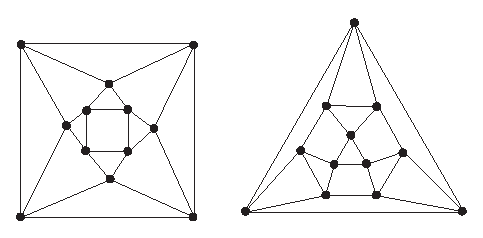
\includegraphics{PS/gfcchcp.eps}
  \caption{The plane graphs $G_{fcc}$ and $G_{hcp}$}
  \label{fig:gfcchcp}
\end{figure}

There is one more tame plane graph that is particularly troublesome.
It is the graph $G_{pent}$\index{pentahedral prism} obtained from
the pictured configuration of twelve balls tangent to a given
central ball (Figure \ref{fig:pentahedral}). (Place a ball at the
north pole, another at the south pole, and then form two pentagonal
rings of five balls.) This case requires individualized attention.
S. Ferguson\index{Ferguson} proves the following theorem in
\shortversion{his thesis \cite{thesis}.}
\longversion{\Part~\ref{part:ferguson}.}

\begin{theorem} [Ferguson] \label{lemma:ferguson}
There are no contravening decomposition stars $D$ whose associated
plane graph is isomorphic to $G_{pent}$.
\end{theorem}


\begin{figure}[htb]
  \centering
  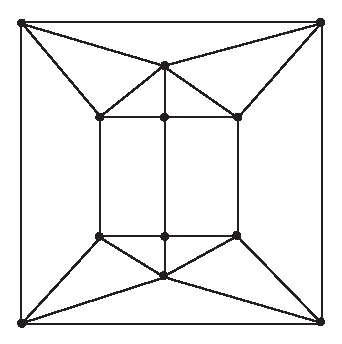
\includegraphics{PS/gpent.eps}
  \caption{The plane graph $G_{pent}$}\index{pentahedral prism}
   of the pentahedral prism.
  \label{fig:pentahedral}
\end{figure}

\section{Logical Skeleton of the Proof}
\label{sec:logic}

Consider the following six claims.  Eventually we will give a
proof of all six statements.  First, we draw out some of their
consequences.  The main results (Theorems~\ref{theorem:kepler},
\ref{theorem:sigma}, and \ref{theorem:sharp}) all follow from
these claims.

\begin{claim}\label{claim-A}
If the maximum of the function $\sigma$ on $\op{DS}$ is $8\,\pt$,
then for every saturated packing $\Lambda$ there exists a
negligible fcc-compatible function $A$.
\end{claim}

\begin{claim}\label{claim-B}
Let $D$ be a contravening decomposition star. Then its plane graph
$G(D)$ is tame.
\end{claim} %\ref{theorem:contravene} in kepler.tex

\begin{claim}\label{claim-C}
If a plane graph is tame, then it is isomorphic to one of the
several thousand plane graphs that appear in the archival list of
plane graphs.
\end{claim} %\ref{theorem:classification} in kepler.tex

\begin{claim}\label{claim-D}
If the plane graph of a contravening
decomposition star is isomorphic to one in the archival list of
plane graphs, then it is isomorphic to one of the following three
plane graphs: $G_{pent}$, $G_{hcp}$, or $G_{fcc}$.
\end{claim} %\label{lemma:fcc-hcp-pent} in linprog.tex

\begin{claim}\label{claim-E}
There do not exist any contravening decomposition stars
$D$ whose associated graph is isomorphic to $G_{pent}$.
\end{claim} %\label{lemma:ferguson} in form.tex

\begin{claim}\label{claim-F}
Contravening decomposition stars exist.
If $D$ is a contravening
decomposition star, and if the plane graph of $D$ is isomorphic to
$G_{fcc}$ or $G_{hcp}$, then $\sigma(D) = 8\,\pt$.  Moreover, up
to Euclidean motion, $U(D)$ is the kissing arrangement of the $12$
balls around a central ball in the face-centered cubic packing or
the kissing arrangement of $12$ balls in the hexagonal-close
packing.
\end{claim} %\label{lemma:local-optimality} in local_opt.tex

Next, we state some of the consequences of these claims.

\begin{lemma}\label{lemma:claim-fcc-graph}
Assume Claims~\ref{claim-B}, \ref{claim-C}, \ref{claim-D}, and
\ref{claim-E}. If $D$ is a contravening decomposition star, then
its plane graph $G(D)$ is isomorphic to $G_{hcp}$ or $G_{fcc}$.
\end{lemma}

\begin{proof} Assume that $D$ is a contravening decomposition
star.  Then its plane graph is tame, and consequently appears on
the archival list of plane graphs.  Thus, it must be isomorphic to
one of $G_{fcc}$, $G_{hcp}$, or $G_{pent}$.  The final graph is
ruled out by Claim~\ref{claim-E}.
\end{proof}

\begin{lemma}\label{lemma:claim-sigma}
Assume Claims~\ref{claim-B}, \ref{claim-C}, \ref{claim-D},
\ref{claim-E}, and \ref{claim-F}. Then Theorem~\ref{theorem:sigma}
holds.
\end{lemma}

\begin{proof}
By Claim~\ref{claim-F} and Lemma~\ref{lemma:claim-fcc-graph}, the
value $8\,\pt$ lies in the range of the function $\sigma$ on
$\op{DS}$.   Assume for a contradiction that there exists a
decomposition star $D\in \op{DS}$ that has $\sigma(D)>8\,\pt$. By
definition, this is a contravening star. By
Lemma~\ref{lemma:claim-fcc-graph}, its plane graph is isomorphic
to $G_{hcp}$ or $G_{fcp}$.  By Claim~\ref{claim-F},
$\sigma(D)=8\,\pt$, in contradiction with $\sigma(D)>8\,\pt$.
\end{proof}

\begin{lemma}\label{lemma:claim-sharp}
Assume Claims~\ref{claim-B}, \ref{claim-C}, \ref{claim-D},
\ref{claim-E}, and \ref{claim-F}.  Then
Theorem~\ref{theorem:sharp} holds.
\end{lemma}

\begin{proof}  By Theorem~\ref{theorem:sigma}, the maximum of
$\sigma$ on $\op{DS}$ is $8\,\pt$.  Let $D$ be a decomposition
star at which the maximum $8\,\pt$ is attained.  Then $D$ is a
contravening star. Lemma~\ref{lemma:claim-fcc-graph} implies that
the plane graph is isomorphic to $G_{hcp}$ or $G_{fcc}$.  The
hypotheses of Claim~\ref{claim-F} are satisfied.  The conclusion
of Claim~\ref{claim-F} is the conclusion of
Theorem~\ref{theorem:sharp}.
\end{proof}

\begin{lemma}
Assume Claims~\ref{claim-A}--\ref{claim-F}. Then the Kepler
conjecture (Theorem~\ref{theorem:kepler}) holds.
\end{lemma}

\begin{proof} As pointed out in Remark~\ref{remark:precise}, the precise
meaning of the Kepler conjecture is for every saturated packing
$\Lambda$, the essential supremum of $\delta(x,r,\Lambda)$ is at
most $\pi/\sqrt{18}$.

Let $\Lambda$ be the set of centers of a saturated packing.  Let
$A:\Lambda \to \ring{R}$ be the negligible, fcc-compatible
function provided by Claim~\ref{claim-A} (and
Lemma~\ref{lemma:claim-sigma}). By Lemma~\ref{lemma:deltabound},
the function $A$ leads to a constant $C$ such that for all $r\ge
1$ and all $x\in \ring{R}^3$, the density $\delta(x,r,\Lambda)$
satisfies
   $$\delta(x,r,\Lambda) \le \pi/\sqrt{18} + C/r.$$
This implies that the essential supremum of $\delta(x,r,\Lambda)$
is at most $\pi/\sqrt{18}$.
\end{proof}

\begin{remark}
One other theorem (Theorem~\ref{lemma:negligible'}) was stated
without proof in Section~\ref{sec:statement}.  This result was
placed there to motivate the other results.  However, it is not an
immediate consequence of Claims~\ref{claim-A}--\ref{claim-F}.  Its
proof appears in Theorem~\ref{lemma:negligible}.
\end{remark}

\section{Proofs of the Central Claims}

The previous section showed that the main results in the
introduction (Theorems~\ref{theorem:kepler}, \ref{theorem:sigma},
and \ref{theorem:sharp}) follow from six claims. This section
indicates where each of these claims is proved, and mentions a few
facts about the proofs.

Claim~\ref{claim-A} is proved in Theorem~\ref{lemma:exista}.
Claim~\ref{claim-B} is proved in Theorem~\ref{theorem:contravene}.
Claim~\ref{claim-C}, the classification of tame graphs, is proved in
Theorem~\ref{theorem:classification}. By the classification of such
graphs, this reduces the proof of the Kepler conjecture to the
analysis of the decomposition stars attached to the finite explicit
list of tame plane graphs.  We will return to Claim~\ref{claim-D} in
a moment.  Claim~\ref{claim-E} is Ferguson's thesis, cited as
Theorem~\ref{lemma:ferguson}.

Claim~\ref{claim-F} is the local optimality of the face-centered
cubic and hexagonal close packings.   In
\Chap~\ref{sec:local-opt}, the necessary local analysis is carried
out to prove Claim~\ref{claim-F} as
Corollary~\ref{lemma:local-optimality2}.

%\begin{lemma}
%A decomposition star whose plane graph is $G_{fcc}$ or $G_{hcp}$ has
%    $$\sigma(D) \le 8\,\pt,$$
%with equality precisely when the decomposition star belongs to
%$\op{DS}_{crit}$. \end{lemma}

%In light of this result, we prove Theorem \ref{theorem:sigma} and
%Theorem \ref{theorem:sharp} by proving that any decomposition star
%whose graph is tame and not equal to $G_{fcc}$ or $G_{hcp}$ is not
%contravening.

Now we return to Claim~\ref{claim-D}. This claim is proved as
Theorem~\ref{lemma:fcc-hcp-pent}.  The idea of the proof is the
following.  Let $D$ be a contravening decomposition star with
graph $G(D)$. We assume that the graph $G(D)$ is not isomorphic to
$G_{fcc}$, $G_{hcp}$, $G_{pent}$ and then prove that $D$ is not
contravening. This is a case-by-case argument, based on the
explicit archival list of plane graphs.

To eliminate these remaining cases, more-or-less generic arguments
can be used.  A linear program is attached to each tame graph $G$.
The linear program can be viewed as a linear relaxation of the
nonlinear optimization problem of maximizing $\sigma$ over all
decomposition stars with a given tame graph $G$. Because it is
obtained by relaxing the constraints on the nonlinear problem, the
maximum of the linear problem is an upper bound on the maximum of
the original nonlinear problem. Whenever the linear programming
maximum is less than $8\,\pt$, it can be concluded that there is
no contravening decomposition star with the given tame graph $G$.
This linear programming approach eliminates most tame graphs.

When a single linear program fails to give the desired bound, it
is broken into a series of linear programming bounds, by branch
and bound techniques.  For every tame plane graph $G$ other than
$G_{hcp}$, $G_{fcc}$, and $G_{pent}$,\index{pentahedral prism} we
produce a series of linear programs that establish that there is
no contravening decomposition star with graph $G$.

The \paper~is organized in the following way.
\Chaps~\ref{sec:construction} through \ref{sec:scoring} introduce
the basic definitions.  \Chap~\ref{sec:scoring} gives a proof of
Claim~\ref{claim-A}. \Chap~\ref{sec:local-opt} proves
Claim~\ref{claim-F}. \longversion{\Chaps~\ref{sec:fine} through
\ref{sec:fb} present the fundamental estimates.}
\Chaps~\ref{sec:def-and-class} through
\ref{sec:proof-classification} give a proof of Claim~\ref{claim-C}.
\Chaps~\ref{sec:startame} through \ref{sec:weight} give a proof of
Claim~\ref{claim-B}. \Chaps~\ref{sec:linearprogram} through
\ref{sec:branchbound} give a proof of Claim~\ref{claim-D}.
Claim~\ref{claim-E} (Ferguson's thesis) \shortversion{is to be
published as a separate paper.} \longversion{appears in
\Part~\ref{part:ferguson}.}


\chapter{Construction of the $Q$-system}
\label{sec:construction}

%This chapter has been written in a way that to be logically independent
%of the other papers in this series.  However, some of the results are
%technical lemmas that are required in other chapters. Thus, some of the
%results in this chapter may seem to be lacking in motivation. For
%motivation and a top-level view of the proof of the Kepler conjecture,
%the reader should consult Chapter~\ref{sec:overview}.  The reader is
%strongly encouraged to read that chapter first.  The paper \cite{CH}
%also gives an informal introduction to the proof that is less
%technically demanding than this paper.

%The ``program" to prove the Kepler conjecture has been changed somewhat
%from some of my earlier papers (see \cite{part1} and \cite{part2}).
%Hence, we do not rely on any definitions or ``program-related'' theorems
%from these papers.  However, we make free use of statements in pure
%geometry from those papers, when it is perfectly clear that these
%statements do not depend on any program-specific definitions or results.
%All program-specific results are proved from scratch in this paper,
%even when the proof is nearly identical to a proof found in one of these
%earlier papers.

It is useful to separate the parts of space of relatively high
packing density from the parts of space with relatively low packing
density.  The $Q$-system, which is developed in this \chap, is a
crude way of marking off the parts of space where the density is
potentially high.  The $Q$-system is a collection of simplices whose
vertices are points of the packing $\Lambda$. The $Q$-system is
reminiscent of the Delaunay decomposition, in the sense of being a
collection of simplices with vertices in $\Lambda$.  In fact, the
$Q$-system is the remnant of an earlier approach to the Kepler
conjecture that was based entirely on the Delaunay decomposition
(see \cite{remarks}).  However, the $Q$-system differs from the
Delaunay decomposition in crucial respects.  The most fundamental
difference is that the $Q$-system, while consisting of
nonoverlapping simplices, does not partition all of space.

This \chap\ defines the set of simplices in the $Q$-system and
proves that they do not overlap.  In order to prove that the
simplices in the $Q$-system do not overlap,  we develop a long
series of lemmas that study the geometry of intersections of
various edges and simplices.  At the end of this \chap, we give
the proof that the simplices in the $Q$-system do not overlap.

\section{Description of the $Q$-system}
\label{sec:Q-describe}



Fix a packing of balls of radius $1$. We identify the packing with
the set $\Lambda$ of its centers.  A packing is thus a subset
$\Lambda$ of $\ring{R}^3$ such that for all $v,w\in\Lambda$,
$|v-w|<2$ implies $v=w$. The centers of the balls are called {\it
\index{vertex} vertices}. The term `vertex' will be reserved for
this technical usage.  A packing is said to be {\it
\index{saturated} saturated\/} if for every $x\in\ring{R}^3$,
there is some $v\in\Lambda$ such that $|x-v|<2$. Any packing is a
subset of a saturated packing. We assume that $\Lambda$ is
saturated. The set $\Lambda$ is countably infinite.

\begin{definition}  We define the {\it truncation parameter}
\index{truncation parameter ($t_0=1.255$)} to be the constant
$t_0=1.255$. It is used throughout. Informal arguments that led to
this choice of constant are described in
\longversion{\Part~\ref{part:intro}}\shortversion{\cite{KC}}.
\end{definition}

Precise constructions that rely on the truncation parameter $t_0$
will appear below.  We will regularly intersect Voronoi cells with
balls of radius $t_0$ to obtain lower bounds on their volumes.  We
will regularly disregard vertices of the packing that lie at
distance greater than $2t_0$ from a fixed $v\in\Lambda$ to obtain
a finite subset of $\Lambda$ (a finite cluster of balls in the
packing) that is easier to analyze than the full packing
$\Lambda$.

The truncation parameter is the first of many decimal constants
that appear. Each decimal constant is an exact rational value,
e.g. $2t_0 = 251/100$.  They are not to be regarded as
approximations of some other value.

\begin{definition}
A {\it quasi-regular\/} triangle\index{quasi-regular triangle} is
a set $T\subset \Lambda$ of three vertices such that if $v,w\in T$
then $|w-v|\le2t_0$. \end{definition}

\begin{definition}
A \index{simplex} simplex\index{simplex} is a set of four
vertices.
%The
%edge-lengths of a simplex $S$ are the lengths $|w-v|$ for $w,v\in
%S$ and $w\ne v$.
A {\it quasi-regular\/} tetrahedron is a simplex $S$ such that if
$v,w\in S$ then $|w-v|\le 2t_0$. A {\it quarter\/} is a simplex
whose edge lengths $y_1,\ldots,y_6$ can be ordered to satisfy
$2t_0\le y_1\le\sqr8$, $2\le y_i\le 2t_0$, $i=2,\ldots,6$. If a
quarter satisfies the strict inequalities $2t_0< y_1< \sqrt8$,
then we say that it is a strict quarter. We call the longest edge
$\{v,w\}$ of a quarter its {\it \index{diagonal} diagonal\/}. When
the quarter is strict, we also say that its diagonal is strict.
When the quarter has a distinguished vertex, the quarter is {\it
upright\/} if the distinguished vertex is an endpoint of the
diagonal, and {\it flat\/} otherwise.
\end{definition}
\index{quarter!strict} \index{quarter!upright}
\index{quarter!flat} \index{quasi-regular}
\index{quasi-regular!triangle} \index{quasi-regular!tetrahedron}

At times, we identify a simplex with its convex hull. We will say,
for example, that the circumcenter of a simplex is contained in
the simplex to mean that the circumcenter is contained in the
convex hull of the four vertices.  Similar remarks apply to
triangles, quasi-regular tetrahedra, quarters, and so forth.  We
will write $|S|$ for the convex hull of $S$ when we wish to be
explicit about the distinction between $|S|$ and its set of
extreme points.

When we wish to give an order on an edge, triangle, simplex, etc.
we present the object as an ordered tuple rather than a set. Thus,
we refer to both $(v_1,\ldots,v_4)$ and $\{v_1,\ldots,v_4\}$ as
simplices, depending on the needs of the given context.

\begin{definition}\index{overlap}
Two manifolds with boundary {\it overlap\/} if their interiors
intersect.
\end{definition}


\begin{definition}  A set $O$ of six vertices is
called a {\it quartered \index{octahedron} octahedron}, if there are
four pairwise nonoverlapping strict quarters $S_1,\ldots,S_4$ all
having the same diagonal, such that $O$ is the union of the four
sets $S_i$ of four vertices.  (It follows easily that the strict
quarters $S_i$ can be given a cyclic order with respect to which
each strict quarter $S_i$ has a face in common with the next, so
that a quartered octahedron is literally a octahedron that has been
partitioned into four quarters.)
\end{definition}

\begin{remark}\label{def:oct-order}
A quartered octahedron may have more than one diagonal of length
less than $\sqr8$, so its decomposition into four strict quarters
need not be unique.  The choice of diagonal has no particular
importance.  Nevertheless, to make things canonical, we pick the
diagonal of length less than $\sqrt8$ with an endpoint of smallest
possible value with respect to the lexicographical ordering on
coordinates; that is, with respect to the ordering $(y_1,y_2,y_3)
< (y_1',y_2',y_3')$, if $y_i=y'_i$, for $i=1,\ldots,k$, and
$y_{k+1}<y'_{k+1}$.  This selection rule for diagonals is fully
translation invariant in the sense that if one octahedron is a
translate of another (whether or not they belong to the same
saturated packing), then the selected diagonal of one is a
translate of the selected diagonal of the other.
\end{remark}

%An {\it octahedral ordering} of a saturated packing is a function
%that assigns a choice of diagonal of length less than $\sqrt8$ to
%each quartered octahedron.  We fix once and for all an octahedral
%ordering of every saturated packing.  We may assume that the
%choice is fully translation invariant in the sense that if
%$\Lambda$ and $\Lambda'$ are any two saturated packings (not
%necessarily distinct) and one contains an octahedron that is a
%translation of an octahedron in the other, then the choice of
%diagonal in one is a translation of the choice in the other.  One
%such (translation invariant) ordering would be the diagonal with
%an endpoint with the smallest possible value with respect to the
%lexicographical ordering on the coordinates.


%This choice of distinguished diagonal is entirely immaterial for
%the proof of the Kepler conjecture.  However, we wish to assert
%that certain constructions are canonical.  For that reason, we
%prefer to avoid basing our choice of diagonal on an arbitrary
%well-ordering of the diagonals. However, there are various rules
%for picking out one diagonal that do not involved any arbitrary
%choices and that rely instead on suitable lexicographical
%orderings of the edge-lengths in the octahedron. A canonical rule
%will be translation and rotation invariant.  Such a rule can be
%designed so that it always selects a diagonal of length less than
%$\sqrt8$ whenever such a diagonal exists.  Of course, any
%canonical rule based on edge-lengths will be invariant under the
%group of isometries of the octahedron, any cannot select a
%distinguished diagonal from a regular octahedron. However, a
%regular octahedron with sides at least $2$ has diagonals of length
%at least $\sqrt8$, and it therefore not a quartered octahedron. To
%avoid excess pedantry, we will not spell out a rule in detail.
% FALSE! Cannot always break the symmetry between the two shorter diags.



\begin{definition} \label{def:anchor}
If $\{v_1,v_2\}$ is an edge of length between $2t_0$ and $\sqr8$,
we say that a vertex $v$ $(\ne v_1,v_2)$ is an {\it \index{anchor}
anchor\/} of $\{v_1,v_2\}$ if its distances to $v_1$ and $v_2$ are
at most $2t_0$.
%
\end{definition}

The two vertices of a quarter that are not on the diagonal are
anchors of the diagonal, and the diagonal may have other anchors
as well.

\begin{definition}\label{def:q-system}
Let $\CalQ$ be the set of quasi-regular tetrahedra and strict
quarters, enumerated as follows. This set is called the
$Q$-system.  It is canonically associated with a saturated packing
$\Lambda$.  (The $Q$ stands for quarters and quasi-regular
tetrahedra.)
%
  \index{Q-system@$Q$-system}


\begin{enumerate}
   \item All quasi-regular tetrahedra.
   \item Every strict quarter such that none of the quarters along
   its diagonal overlaps any other
   quasi-regular tetrahedron or strict quarter.
   \item Every strict quarter whose diagonal has four or more
   anchors, as long as there are not exactly four anchors arranged
   as a quartered
   octahedron.
   \item The fixed choice of four strict quarters in each
   quartered octahedron.
   %\item Assume a strict quarter does not overlap a quasi-regular tetrahedron,
   %overlaps at least one other strict quarter,
   % and is not part of a quartered octahedron.  Of these, we include
   %\begin{enumerate}
   \item Every strict quarter $\{v_1,v_2,v_3,v_4\}$ whose diagonal
      $\{v_1,v_3\}$ has exactly three anchors $v_2$, $v_4$, $v_5$ provided that
      the following hold (for some choice of indexing).
      (a) $\{v_2,v_5\}$ is a strict diagonal
      with exactly three anchors: $v_1$, $v_3$, $v_4$.
      (b) $d_{24}+d_{25}>\pi$, where $d_{24}$ is the dihedral angle
       of the simplex $\{v_1,v_3,v_2,v_4\}$ along the edge $\{v_1,v_3\}$
       and $d_{25}$ is the dihedral angle of the simplex
       $\{v_1,v_3,v_2,v_5\}$ along the edge $\{v_1,v_3\}$.
       %The sum of the dihedral
       %  angles $\dih(v_1,v_3,v_2,v_4)+\dih(v_1,v_3,v_2,v_5)$ is
       %  greater than $\pi$.
   %\end{enumerate}
\end{enumerate}
No other quasi-regular tetrahedra or strict quarters are included
in the $Q$-system $\CalQ$.
\end{definition}


The following theorem is the main result of this \chap.

\begin{theorem}\label{thm:nonoverlap}
For every saturated packing, there exists a uniquely determined
$Q$-system.  Distinct simplices in the $Q$-system have disjoint
interiors.
\end{theorem}

While proving the theorem, we give a complete classification of
the various ways in which one quasi-regular tetrahedron or strict
quarter can overlap another.

Having completed our primary purpose of showing that the simplices
in the $Q$-system do not overlap, we state the following small
lemma. It is an immediate consequence of the definitions, but
which is nonetheless useful in the \chaps\ that follow.

\begin{lemma} \label{lemma:diags-engulf}
If one quarter along a diagonal lies in the $Q$-system, then all
quarters along the diagonal lie in the $Q$-system.
\end{lemma}

\begin{proof} This is true by construction.  Each of the defining properties
of a quarter in the $Q$-system is true for one quarter along a
diagonal if and only if  it is true of all quarters along the
diagonal.
\end{proof}


\section{Geometric Considerations}
    \label{sec:decomposition}

\begin{remark}  The primary definitions and
constructions of this paper are translation invariant.  That is,
if $\lambda\in\ring{R}^3$ and $\Lambda$ is a saturated packing,
then $\lambda+\Lambda$ is a saturated packing.  If
$A:\Lambda\to\ring{R}$ is a negligible fcc-compatible function for
$\Lambda$, then $\lambda+v\mapsto A(v)$ is a negligible
fcc-compatible function for $\lambda+\Lambda$.  If $\CalQ$ is the
$Q$-system of $\Lambda$, then $\lambda+\CalQ$ is the $Q$-system of
$\lambda+\Lambda$. Because of general translational invariance,
when we fix our attention on a particular $v\in\Lambda$, we will
often assume (without loss of generality) that the coordinate
system is fixed in such a way that $v$ lies at the origin.
\end{remark}

Our simplices are generally assumed to come labeled with a
distinguished vertex, fixed  at the origin. (The origin will
always be at a vertex of the packing.) We number the edges of each
simplex $1,\ldots,6$, so that edges $1$, $2$, and $3$ meet at the
origin, and the edges $i$ and $i+3$ are opposite, for $i=1,2,3$.
(See Figure~\ref{fig:diag11}.)  $S(y_1,y_2,\ldots,y_6)$ denotes a
simplex whose edges have lengths $y_i$, indexed in this way. We
refer to the endpoints away from the origin of the first, second,
and third edges as the first, second, and third vertices.
%
 \index{labels!edge}
 \index{first!edge}

\begin{definition}\label{def:dih}
In general, let $\dih(S)$ be the dihedral angle of a simplex $S$
along its first edge. When we write a simplex in terms of its
vertices $(w_1,w_2,w_3,w_4)$, then $\{w_1,w_2\}$ is understood to
be the first edge.
%
 \index{dih (dihedral angle)}
\end{definition}

\begin{definition}
We define the {\it radial projection\/} of a set $X$ to be the
radial projection $x\mapsto x/|x|$ of $X\setminus{0}$ to the unit
sphere centered at the origin. We say the two sets {\it cross\/}
if their radial projections to the unit sphere
overlap.\index{projection of a set}
%
 \index{cross}
 \index{radial projection}
\end{definition}


\begin{definition}
    \label{def:calE}
If $S$ and $S'$ are nonoverlapping simplices with a shared face $F$,
we define $\CalE(S,S')$ as the distance between the two vertices
(one on $S$ and the other on $S'$) that do not lie on $F$.  We may
express this as a function
   $$\CalE(S,S')=\CalE(S(y_1,\ldots,y_6),y_1',y_2',y_3')$$
of nine variables, where $S=S(y_1,\ldots,y_6)$  and
$S'=S(y_1',y_2',y_3',y_4,y_5,y_6)$, positioned so that $S$ and $S'$
are nonoverlapping simplices with a shared face $F$ of edge-lengths
$(y_4,y_5,y_6)$.   The function of nine variables is defined only
for values $(y_i,y_i')$ for which the simplices $S$ and $S'$ exist.
(Figure~\ref{fig:diag11}).
\end{definition}

\begin{figure}[htb]
  \centering
  \includegraphics{PS/calE.eps}
  \caption{$\CalE$ measures the distance between the vertices at $0$ and $v$.
   The standard indexing of the edges of a simplex
   is marked on the lower simplex.}
  \label{fig:diag11}
\end{figure}

Several lemmas in this paper rely on calculations of lower bounds
to the function $\CalE$ in the special case when the edge between
the vertices $0$ and $v$ passes through the shared face $F$. If
intervals containing $y_1,\ldots,y_6,y_1',y_2',y_3'$ are given,
then lower bounds on $\CalE$ over that domain are generally easy
to obtain.  Detailed examples of calculations of the lower bound
of this function can be found in \cite[Sec. 4]{part1}.

To work one example, we suppose we are asked to give a lower bound
on $\CalE$ when the simplex $S=S(y_1,\ldots,y_6)$ satisfies
$y_i\ge2$ and $y_4,y_5,y_6\le 2t_0$ and
$S'=S(y'_1,y'_2,y'_3,y_4,y_5,y_6)$ satisfies $y'_i\ge2$, for
$i=1,\ldots,3$. Assume that the edge $\{0,v\}$ passes through the
face shared between $S$ and $S'$, and that $|v|<\sqrt8$, where $v$
is the vertex of $S'$ that is not on $S$.  We claim that any pair
$S,S'$ can be deformed by moving one vertex at a time until $S$ is
deformed into $S(2,2,2,2t_0,2t_0,2t_0)$ and $S'$ is deformed into
$S(2,2,2,2t_0,2t_0,2t_0)$.  Moreover, these deformations preserve
the constraints (including that $\{0,v\}$ passes through the shared
face), and is non-increasing in $|v|$.  From the existence of this
deformation, it follows that the original $|v|$ satisfies
   $$|v| \ge \CalE(S(2,2,2,2t_0,2t_0,2t_0),2,2,2).$$

We produce the deformation in this case as follows. We define the
{\it pivot\/} of a vertex $v$ with respect to two other vertices
$\{v_1,v_2\}$ as the circular motion of $v$ held at a fixed
distance from $v_1$ and $v_2$, leaving all other vertices fixed.
The {\it axis\/}\index{axis} of the \index{pivot} pivot is the
line through the two fixed vertices. Each pivot of a vertex can
move in two directions.  Let the vertices of $S$ be
$\{0,v_1,v_2,v_3\}$, labeled so that $|v_i|=y_i$.  Let
$S'=\{v,v_1,v_2,v_3\}$.  We pivot $v_1$ around the axis through
$0$ and $v_2$. By picking a suitable direction for the pivot,
$v_1$ moves away from $v$ and $v_3$. Its distance to $0$ and $v_2$
remains fixed. We continue with this circular motion until
$|v_1-v_3|$ achieves its upper bound or the segment $\{v_1,v_3\}$
intersects the segment $\{0,v\}$ (which threatens the constraint
that the segment $\{0,v\}$ pass through the common face).  (We
leave it as an exercise\footnote{Compare
Lemma~\ref{lemma:no-pass-sqrt2}.} to check that the second
possibility cannot occur because of the edge length upper bounds
on both diagonals of $\sqrt8$.  That is, there does not exist a
convex planar quadrilateral with sides at least $2$ and diagonals
less than $\sqrt8$.) Thus, $|v_1-v_3|$ attains its constrained
upper bound $2t_0$. Similar pivots to $v_2$ and $v_3$ increase the
lengths $|v_1-v_2|$, $|v_2-v_3|$, and $|v_3-v_1|$ to $2t_0$.
Similarly, $v$ may be pivoted around the axis through $v_1$ and
$v_2$ so as to decrease the distance to $v_3$ and $0$ until the
lower bound of $2$ on $|v-v_3|$ is attained.  Further pivots
reduce all remaining edge lengths to $2$.   In this way, we obtain
a rigid figure realizing the absolute lower bound of $|v|$.  A
calculation with explicit coordinates gives $|v|>2.75$.

Because lower bounds are generally easily determined from a series
of pivots through arguments such as this one, we will state them
without proof. We will state that these bounds were obtained by
{\it geometric considerations}, to indicate that the bounds were
obtained by the deformation arguments of this paragraph.
\index{geometric considerations}


\section{Incidence Relations}


\begin{lemma} \label{lemma:v-interior-alt}
Let $v,v_1,v_2,v_3$, and $v_4$ be distinct points in $\ring{R}^3$
with pairwise distances at least $2$.  Suppose that $|v_i-v_j|\le
2t_0$ for $i\ne j$ and $\{i,j\}\ne\{1,4\}$. Then $v$ does not lie
in the convex hull of $\{v_1,v_2,v_3,v_4\}$.
\end{lemma}

\begin{proof}
This lemma is proved in~\cite[Lemma 3.5]{part1}.
\end{proof}



\begin{lemma} \label{lemma:v-interior}
Let $S$ be a simplex whose edges have length between $2$ and
$2\sqrt2$.  Suppose that $v$ has distance at least $2$ from each
of the vertices of $S$.  Then $v$ does not lie in the convex hull
of $S$.
\end{lemma}

\begin{proof} Assume for a contradiction that $v$ lies in the
convex hull of $S$.   Place a unit sphere around $v$.  The simplex
$S$ partitions the unit sphere into four spherical triangles,
where each triangle is the intersection of the unit sphere with
the cone over a face of $S$, centered at $v$.   By the constraints
on the lengths of edges, the arclength of each edge of the
spherical triangle is at most $\pi/2$.  ($\pi/2$ is attained when
$v$ has distance $2$ to two of the vertices, and these two
vertices have distance $2\sqrt2$ between them.)  A spherical
triangle with edges of arclength at most $\pi/2$ has area at most
$\pi/2$.  In fact, any such spherical triangle can be placed
inside a octant of the unit sphere, and each octant has area
$\pi/2$. This partitions the sphere of area $4\pi$ into four
regions of area at most $\pi/2$. This is absurd.
\end{proof}

\bigskip
\begin{corollary}\label{cor:interior}
%{Lemma 1.2}
No vertex of the packing is contained in the convex hull of a
quasi-regular tetrahedron or quarter (other than the vertices of
the simplex).
\end{corollary}

\begin{proof}
The corollary is immediate.
\end{proof}


\begin{definition} \label{def:passes-through}
Let $v_1,v_2,w_1,w_2,w_3\in\Lambda$ be distinct.  We say that an
edge $\{v_1,v_2\}$ {\it passes through} the triangle
$\{w_1,w_2,w_3\}$ if the convex hull of $\{v_1,v_2\}$ meets some
point of the convex hull of $\{w_1,w_2,w_3\}$ and if that point of
intersection is not any of the extreme points $v_1$, $v_2$, $w_1$,
$w_2$, $w_3$.
%
 \index{passes through}
\end{definition}

\begin{lemma} \label{lemma:2t0-doesnt-pass-through}
%\proclaim{Lemma 1.3}
An edge of length $2t_0$ or less cannot pass through a triangle
whose edges have lengths $2t_0$, $2t_0$, and $\sqr8$ or less.
\end{lemma}

\begin{proof}  The distance between each pair of vertices is at least 2.
Geometric considerations show that the edge has length at least
$${\CalE}(S(2,2,2,2t_0,2t_0,\sqr8),2,2,2) > 2t_0.$$
\end{proof}

\begin{definition}\label{def:eta}\index{circumradius}
%
 \index{Zeta@$\eta$}
Let $\eta(x,y,z)$ denote the circumradius of a
triangle with edge-lengths $x$, $y$, and $z$.
\end{definition}


\begin{lemma}
\label{lemma:no-pass-sqrt2}
%{\bf Lemma I 3.2.}
Suppose that the circumradius of $\{v_1,v_2,v_3\}$ is less than
$\sqrt2$. Then an edge $\{w_1,w_2\}\subset\Lambda$ of length at
most $\sqr8$ cannot pass through the face.
\end{lemma}

\begin{proof}  Assume for a contradiction that $\{w_1,w_2\}$ passes through the
triangle $\{v_1,v_2,v_3\}$.   By geometric considerations, the
minimal length for $\{w_1,w_2\}$ occurs when $|w_i-v_j|=2$, for
$i=1,2$, $j=1,2,3$.  This distance constraint places the
circumscribing circle of $\{v_1,v_2,v_3\}$ on the sphere of radius
$2$ centered at $w_1$ (resp. $w_2$).  If $r<\sqrt2$ is the
circumradius of $\{v_1,v_2,v_3\}$, then for this extremal
configuration we have the contradiction
    $$\sqrt8\ge |w_1-w_2| = 2\sqrt{4-r^2}>\sqrt8.$$
\end{proof}

\begin{lemma} \label{lemma:qrtet-pair-pass}
%{Lemma 1.4}
If an edge of length at most $\sqrt{8}$ passes through a
quasi-regular triangle, then each of the two endpoints of the edge
is at most $2.2$ away from each of the vertices of the triangle
(see Figure~\ref{fig:dia31}).\index{quasi-regular!triangle}
\end{lemma}

\begin{figure}[htb]
  \centering
  \includegraphics{PS/dia31.ps}
  \caption{Frame (a) depicts two quasi-regular tetrahedra that share
  a face.  The same convex body may also be viewed as three quarters
  that share a diagonal, as in Frame (b).}
  \label{fig:dia31}
\end{figure}


\begin{proof}
Let the diagonal edge be $\{v_0,v_0'\}$ and the vertices of the
face be $\{v_1,v_2,v_3\}$.  If $|v_i-v_0|>2.2$ or $|v_i-v_0'|>2.2$
for some $i>0$, then geometric considerations give the
contradiction
$$|v_0-v_0'|\ge{\CalE}(S(2,2,2,2t_0,2t_0,2t_0),2,2,2.2) > \sqr8.$$
\end{proof}

%\begin{lemma}\label{lemma:2.15}
%Let $\{v_1,v_2,v_3\}$ be a quasi-regular triangle.  Assume that there is
%a vertex $v$ such that the distance from $v$ to the circumcenter is less
%than the circumradius.  Then $|v-v_i|\le2.15$, for $i=1,2,3$.  In
%particular, $\{v,v_1,v_2,v_3\}$ is a quasi-regular tetrahedron.
%\end{lemma}
%
%\begin{proof} This is proved in \cite[Lemma~3.4]{part1}.
%\end{proof}

\begin{lemma}\label{lemma:qrtet-quarter}
Suppose $S$ and $S'$ are quasi-regular tetrahedra that share a
face.  Suppose that the edge $e$ between the two vertices that are
not shared has length at most $\sqrt8$.   Then the convex hull of
$S$ and $S'$ consists of three quarters with diagonal $e$.  No
other quarter overlaps $S$ or $S'$.
\end{lemma}

\begin{proof}
Suppose that $S$ and $S'$ are adjacent quasi-regular tetrahedra
with a common face $F$.   By the
Lemma~\ref{lemma:qrtet-pair-pass}, each of the six external faces
of this pair of quasi-regular tetrahedra has circumradius at most
$\eta(2.2,2.2,2t_0)<\sqr2$. A diagonal of a quarter  cannot pass
through a face of this size by Lemma~\ref{lemma:no-pass-sqrt2}.
This implies that no other quarter overlaps these quasi-regular
tetrahedra.
\end{proof}


\begin{lemma} \label{lemma:pass-anchor}
%\proclaim{Lemma 1.5}
Suppose an edge $\{w_1,w_2\}$ of length at most $\sqr8$ passes
through the face formed by a diagonal $\{v_1,v_2\}$ and one of its
anchors. Then $w_1$ and $w_2$ are also anchors of $\{v_1,v_2\}$.
\end{lemma}

\begin{proof}  This follows from
the inequality
  $${\CalE}(S(2,2,2,\sqr8,2t_0,2t_0),2,2,2t_0) > \sqr8$$
and geometric considerations.
\end{proof}


\begin{definition} \label{def:height}  Let $\Lambda$ be a
saturated packing.  Assume that the coordinate system is fixed in
such a way that the origin is a vertex of the packing.  The {\it
height\/} of a vertex is its distance from the
origin.
%
 \index{height}
\end{definition}

\begin{definition} \label{def:enclosed}\index{enclosed}
We say that a vertex is {\it enclosed\/} over a figure
if it lies in the interior of the
cone at the origin generated by the figure.
%
 \index{vertex!enclosed}\index{enclosed}
\end{definition}


\begin{definition} \label{def:corner}
An {\it adjacent pair of quarters} consists of two quarters
sharing a face along a common diagonal. The common vertex that
does not lie on the diagonal is called the {\it base point\/} of
the adjacent pair.  (When one of the quarters comes with a marked
distinguished vertex, we do {\it not\/} assume that this marked
vertex coincides with the base point of the pair.)  The other four
vertices are called the {\it corners\/}  of the configuration.
%
 \index{adjacent pair}
 \index{base point}
 \index{corner}
\end{definition}

\begin{definition}
If the two corners, $v$ and $w$, that do not lie on the diagonal
satisfy $|w-v|<\sqrt8$, then the base point and four corners can
be considered as an adjacent pair in a second way, where $\{v,w\}$
functions as the diagonal.  In this case we say that the original
diagonal and the diagonal $\{v,w\}$ are {\it conflicting
diagonals}.\index{conflicting diagonal} %
\end{definition}

\begin{definition}
A quarter is said to be {\it isolated}\index{isolated} if it
is not part of an adjacent pair.  Two isolated quarters that
overlap are said to form an {\it isolated
pair}.\index{pair!isolated}
%
\end{definition}

\begin{lemma} \label{lemma:skew-quad}
%\proclaim{Lemma 1.6}
Suppose that there exist four nonzero vertices $v_1,\ldots,v_4$ of
height at most $2t_0$ (that is, $|v_i|\le 2t_0$) forming a skew
quadrilateral. Suppose that the diagonals $\{v_1,v_3\}$ and
$\{v_2,v_4\}$ have lengths between $2t_0$ and $\sqr8$. Suppose the
diagonals $\{v_1,v_3\}$ and $\{v_2,v_4\}$ cross. Then the four
vertices are the corners of an adjacent pair of quarters with base
point at the origin.
\end{lemma}

\begin{proof}
 Set $d_1=|v_1-v_3|$ and $d_2 = |v_2-v_4|$.
By hypothesis, $d_1$ and $d_2$ are at most $\sqr8$.
 If $|v_1-v_2|>2t_0$,
geometric considerations give the contradiction
    $$\max(d_1,d_2)\ge \CalE(S(2t_0,2,2,2t_0,\sqr8,2t_0),2,2,2) > \sqr8
    \ge\max(d_1,d_2).$$
Thus, $\{0,v_1,v_2\}$ is a quasi-regular triangle,  as are
$\{0,v_2,v_3\}$, $\{0,v_3,v_4\}$, and $\{0,v_4,v_1\}$ by symmetry.
\end{proof}

\begin{lemma} \label{lemma:oct}
%\proclaim{Lemma 1.7}
If, under the same hypotheses as Lemma~\ref{lemma:skew-quad},
there is a vertex $w$ of height at most $\sqr8$ enclosed over the
adjacent pair of quarters, then $\{0,v_1,\ldots,v_4,w\}$ is a
quartered octahedron.
\end{lemma}


\begin{proof}
 If the enclosed $w$ lies over say $\{0,v_1,v_2,v_3\}$, then
$|w-v_1|$, $|w-v_3|\le 2t_0$ (Lemma~\ref{lemma:pass-anchor}), where
$\{v_1,v_3\}$ is a diagonal. Similarly, the distance from $w$ to the
other two corners is at most $2t_0$.
\end{proof}

\begin{lemma} \label{lemma:double-face}
%proclaim{Lemma 1.8}
Let $v_1$ and $v_2$ be anchors of $\{0,w\}$ with $2t_0\le |w|\le
\sqr8$. If an edge $\{v_3,v_4\}$ passes through both faces,
$\{0,w,v_1\}$ and $\{0,w,v_2\}$, then $|v_3-v_4|>\sqr8$.
\end{lemma}

\begin{proof}
Suppose the figure exists with $|v_3-v_4|\le\sqr8$. Label vertices
so $v_3$ lies on the same side of the figure as $v_1$. Contract
$\{v_3,v_4\}$ by moving $v_3$ and $v_4$ until
    $\{v_i,u\}$ has length $2$,
for $u=0,w,v_{i-2}$, and $i=3,4$. Pivot $w$ away from $v_3$ and
$v_4$ around the axis $\{v_1,v_2\}$ until
    $|w|=\sqr8$.
Contract $\{v_3,v_4\}$ again. By stretching $\{v_1,v_2\}$, we
obtain a square of edge two and vertices $\{0,v_3,w,v_4\}$. Short
calculations based on explicit formulas for the dihedral angle and
its partial derivatives give
    \begin{equation}
        \dih(S(\sqr8,2,y_3,2,y_5,2)) > 1.075,\quad
        y_3,y_5\in[2,2t_0],\label{eqn:1.7.1}
    \end{equation}
    %
    \begin{equation}
    \dih(S(\sqr8,y_2,y_3,2,y_5,y_6)) >1,\quad
        y_2,y_3,y_5,y_6\in[2,2t_0].
        \label{eqn:1.7.2}
    \end{equation}
Then
$$\pi\ge \dih(0,w,v_3,v_1) + \dih(0,w,v_1,v_2) + \dih(0,w,v_2,v_4)
    > 1.075 + 1 + 1.075 > \pi.$$
Therefore, the figure does not exist.
\end{proof}

\begin{lemma} \label{lemma:single-enclosed}
%proclaim{Lemma 1.11}
Two vertices $w,w'$ of height at most $\sqr8$ cannot be enclosed
over a triangle $\{v_1,v_2,v_3\}$ satisfying $|v_1-v_2|\le\sqrt8$,
$|v_1-v_3|\le 2t_0$, and $|v_2-v_3|\le 2t_0$.
\end{lemma}

\begin{proof}
For a contradiction, assume the figure exists. The long edge
$\{v_1,v_2\}$ must have length at least $2t_0$ by
Lemma~\ref{lemma:qrtet-pair-pass}. This diagonal has anchors
$\{0,v_3,w,w'\}$. Assume that the cyclic order of vertices around
the line $\{v_1,v_2\}$ is $0,v_3,w,w'$. We see that $\{v_1,w\}$ is
too short to pass through $\{0,v_2,w'\}$, and $w$ is not inside
the simplex $\{0,v_1,v_2,w'\}$.  Thus, the projections of the
edges $\{v_2,w\}$ and $\{0,w'\}$ to the unit sphere at $v_1$ must
intersect.  It follows that $\{0,w'\}$ passes through
$\{v_1,v_2,w\}$ or $\{v_2,w\}$ passes through $\{v_1,0,w'\}$.  But
$\{v_2,w\}$ is too short to pass through $\{v_1,0,w'\}$.  Thus,
$\{0,w'\}$ passes through both $\{v_1,v_2,w\}$ and
$\{v_1,v_2,v_3\}$. Lemma~\ref{lemma:double-face} gives the
contradiction $|w'|>\sqrt8$.
\end{proof}

\begin{lemma} \label{lemma:pass-makes-quarter}
%{Lemma 1.9}
Let $v_1,v_2,v_3$ be anchors of $\{0,w\}$, where
$2t_0\le|w|\le\sqr8$, $|v_1-v_3|\le\sqr8$, and the edge
$\{v_1,v_3\}$ passes through the face $\{0,w,v_2\}$.  Then
$\min(|v_1-v_2|,|v_2-v_3|)\le2t_0$. Furthermore, if the minimum is
$2t_0$, then $|v_1-v_2|=|v_2-v_3|=2t_0$.
\end{lemma}

\begin{proof}
Assume $\min\ge2t_0$. As in the proof of
Lemma~\ref{lemma:double-face}, we may assume that $(0,v_1,w,v_3)$
is a square.  We may also assume, without loss of generality, that
$|w-v_2|=|v_2|=2t_0$. This forces $|v_2-v_i|=2t_0$, for $i=1,3$.
This is rigid,  and is the unique figure that satisfies the
constraints. The lemma follows.
\end{proof}


\bigskip

\section{Overlap of Simplices}
\label{sec:nonoverlap}

This section gives a proof of Theorem~\ref{thm:nonoverlap}
(simplices in the $Q$-system do not overlap).  This is accomplished
in a series of lemmas.  The first of these treats quasi-regular
tetrahedra.


\begin{lemma} \label{lemma:qrtet-over}
A quasi-regular tetrahedron does not overlap any
other simplex in the $Q$-system.
\end{lemma}

\begin{proof} Edges of quasi-regular tetrahedra are too short to
pass through the face of another quasi-regular tetrahedron or
quarter (Lemma~\ref{lemma:2t0-doesnt-pass-through}).  If a
diagonal of a strict quarter passes through the face of a
quasi-regular tetrahedron, then Lemma~\ref{lemma:qrtet-quarter}
shows that the strict quarter is one of three joined along a
common diagonal.  This is not one of the enumerated types of
strict quarter in the $Q$-system.
\end{proof}

\begin{lemma} \label{lemma:oct-over}
A quarter in the $Q$-system that is part of a
quartered octahedron does not overlap any other simplex in the
$Q$-system.
\end{lemma}

\begin{proof} By construction, the quarters that lie along a
different diagonal of the octahedron do not belong to the
$Q$-system.  Edges of length at most $2t_0$ are too short to pass
through an external face of the octahedron
(Lemma~\ref{lemma:2t0-doesnt-pass-through}). A diagonal of a
strict quarter cannot pass through an external face either,
because of Lemma~\ref{lemma:qrtet-pair-pass}.
\end{proof}

\begin{lemma}\label{lemma:adj-over}
Let $Q$ be a strict quarter that is part of an adjacent pair.
Assume that $Q$ is not part of a quartered octahedron.  If $Q$
belongs to the $Q$-system, then it does not overlap any other
simplex in the $Q$-system.
\end{lemma}

The proof of this lemma will give valuable details about how one
strict quarter overlaps another.

\begin{proof}
Fix the origin at the base point of an adjacent pair of quarters.
We investigate the local geometry when another quarter overlaps
one of them.  (This happens, for example, when there is a
conflicting diagonal in the sense of Definition~\ref{def:corner}.)

%if both diagonals between opposite corners of the adjacent pair of
%quarters have lengths at most $\sqr8$.  We will see that a
%conflict like this between the diagonals between corners is the
%only way an adjacent pair of quarters can overlap another quarter.
%We call these {\it conflicting\/} diagonals.

Label the base point of the pair of quarters $v_0$, and the four
corners  $v_1$, $v_2$, $v_3$, $v_4$, with $\{v_1,v_3\}$ the common
diagonal. Assume that $|v_1-v_3|<\sqrt8$.\index{conflicting
diagonals}

If two quarters overlap then a face on one of them overlaps a face
on the other.  By Lemmas~\ref{lemma:single-enclosed} and
\ref{lemma:double-face}, we actually have that some edge (in fact
the diagonal) of each passes through a face of the other.  This
edge cannot exit through another face by
Lemma~\ref{lemma:double-face} and it cannot end inside the simplex
by Corollary~\ref{cor:interior}. Thus, it must end at a vertex of
the other simplex.  We break the proof into cases according to
which vertex of the simplex it terminates at. In Case 1, the edge
has the base point as an endpoint.  In Case 2, the edge has a
corner as an endpoint.

\noindent{\bf Case 1.} {\it The edge $\{0,w\}$ passes through the
triangle $\{v_1,v_2,v_3\}$, where $\{0,w\}$ is a diagonal of a
strict quarter.}

Lemma~\ref{lemma:pass-anchor} implies that $v_1$ and $v_3$ are
anchors of $\{0,w\}$. The only other possible anchors of $\{0,w\}$
are $v_2$ or $v_4$, for otherwise an edge of length at most $2t_0$
edge passes through a face formed by $\{0,w\}$ and one of its
anchors. If both $v_2$ and $v_4$ are anchors, then we have a
quartered octahedron, which has been excluded by the hypotheses of
the lemma.  Otherwise, $\{0,w\}$ has at most $3$ anchors: $v_1$,
$v_3$, and either $v_2$ or $v_4$. In fact, it must have exactly
three anchors, for otherwise there is no quarter along the edge
$\{0,w\}$. So there are exactly two quarters along the edge
$\{0,w\}$. There are at least four anchors along $\{v_1,v_3\}$:
$0$, $w$, $v_2$, and $v_4$.  The quarters along the diagonal
$\{v_1,v_3\}$ lie in the $Q$-system. (None of these quarters is
isolated.)  The other two quarters, along the diagonal $\{0,w\}$,
are not in the $Q$-system. They form an adjacent pair of quarters
(with base point $v_4$ or $v_2$) that has conflicting diagonals,
$\{0,w\}$ and $\{v_1,v_3\}$, of length at most $\sqr8$.

\noindent {\bf Case 2.}  {\it $\{v_2,v_4\}$ is a diagonal of
length less than $\sqr8$ (conflicting with $\{v_1,v_3\}$).}

(Note that if an edge of a quarter passes through the shared face
of an adjacent pair of quarters, then that edge must be
$\{v_2,v_4\}$, so that Case 1 and Case 2 are exhaustive.) The two
diagonals $\{v_1,v_3\}$ and $\{v_2,v_4\}$ do not overlap. By
symmetry, we may assume that $\{v_2,v_4\}$ passes through the face
$\{0,v_1,v_3\}$. Assume (for a contradiction) that both diagonals
have an anchor other than $0$ and the corners $v_i$. Let the
anchor of $\{v_2,v_4\}$ be denoted $v_{24}$ and that of
$\{v_1,v_3\}$ be $v_{13}$. Assume the figure is not a quartered
octahedron, so that $v_{13}\ne v_{24}$. By
Lemma~\ref{lemma:2t0-doesnt-pass-through}, it is impossible to
draw the edges $\{v_1,v_{13}\}$ and $\{v_{13},v_3\}$ between $v_1$
and $v_3$.  In fact, if the edges pass outside the quadrilateral
$\{0,v_2,v_{24},v_4\}$, one of the edges of length at most $2t_0$
(that is,
    $\{0,v_2\}$, $\{v_2,v_{24}\}$, $\{v_{24},v_4\}$,
or $\{v_4,0\}$) violates the lemma applied to the face
$\{v_1,v_3,v_{13}\}$. If they pass inside the quadrilateral, one of the
edges $\{v_1,v_{13}\}$, $\{v_{13},v_3\}$ violates the lemma applied to
the face
    $\{0,v_{2},v_4\}$ or $\{v_{24},v_2,v_4\}$.
We conclude that at most one of the two diagonals has additional
anchors.

If neither of the two diagonals has more than three anchors, we
have nothing more than two overlapping adjacent pairs of quarters
along conflicting diagonals.  The two quarters along the lower
edge $\{v_2,v_4\}$ lie in the $Q$-system.  Another way of
expressing this ``lower-edge'' condition is to require the two
adjacent quarters $Q_1$ and $Q_2$ satisfy
$\dih(Q_1)+\dih(Q_2)>\pi$, when the dihedral angles are measured
along the diagonal. The pair $(Q_1',Q_2')$ along the upper edge
will have $\dih(Q_1')+\dih(Q_2')<\pi$.

If there is a diagonal with more than three anchors,  the quarters
along the diagonal with more than three anchors lie in the
$Q$-system.  Any additional quarters along the diagonal
$\{v_2,v_4\}$ belong to an adjacent pair. Any additional quarters
along the diagonal $\{v_1,v_3\}$ cannot intersect the adjacent
pair along $\{v_2,v_4\}$.  Thus, every quarter intersecting an
adjacent pair also belongs to an adjacent pair.

In both possibilities of case 2, the two quarters left out of the
$Q$-system correspond to a conflicting diagonal.
\end{proof}

\begin{remark}\label{remark:iso}
We have seen in the proof of the Lemma~\ref{lemma:adj-over} that
if a strict quarter $Q$ overlaps a strict quarter that is part of
an adjacent pair, then $Q$ is also part of an adjacent pair. Thus,
if an isolated strict quarter overlaps another strict quarter,
then both strict quarters are necessarily isolated.
\end{remark}

\begin{lemma}\label{lemma:iso-over}
If an isolated strict quarter $Q$ overlaps another strict quarter,
then the diagonal of $Q$ has exactly three anchors.
\end{lemma}

The proof of the lemma will give detailed information about the
geometrical configuration that is obtained when an isolated
quarter overlaps another strict quarter.

\begin{proof}  Assume that there are two strict quarters $Q_1$ and $Q_2$
that overlap.  Following Remark~\ref{remark:iso}, assume that
neither is adjacent to another quarter. Let $\{0,u\}$ and
$\{v_1,v_2\}$ be the diagonals of $Q_1$ and $Q_2$. Suppose the
diagonal $\{v_1,v_2\}$ passes through a face $\{0,u,w\}$ of $Q_1$.
By Lemma~\ref{lemma:pass-anchor}, $v_1$ and $v_2$ are anchors of
$\{0,u\}$. Again, either the length of $\{v_1,w\}$ is at most
$2t_0$ or the length of $\{v_2,w\}$ is at most $2t_0$, say
$\{w,v_2\}$ (by Lemma~\ref{lemma:pass-makes-quarter}). It follows
that
    $Q_1=\{0,u,w,v_2\}$ and $|v_1-w|\ge2t_0$.
($Q_1$ is not adjacent to another quarter.)  So $w$ is not an anchor of
$\{v_1,v_2\}$.

Let $\{v_1,v_2,w'\}$ be a face of $Q_2$ with $w'\ne 0,u$. If
$\{v_1,w',v_2\}$ does not link $\{0,u,w\}$, then $\{v_1,w'\}$ or
$\{v_2,w'\}$ passes through the face $\{0,u,w\}$, which is
impossible by Lemma~\ref{lemma:2t0-doesnt-pass-through}. So
$\{v_1,v_2,w'\}$  links $\{0,u,w\}$ and an edge of $\{0,u,w\}$
passes through the face $\{v_1,v_2,w'\}$. It is not the edge
$\{u,w\}$ or $\{0,w\}$, for they are too short by
Lemma~\ref{lemma:2t0-doesnt-pass-through}.  So $\{0,u\}$ passes
through $\{w',v_1,v_2\}$. The only anchors of $\{v_1,v_2\}$ (other
than $w'$) are $u$ and $0$ (by Lemma~\ref{lemma:double-face}).
Either $\{u,w'\}$ or $\{w',0\}$ has length at most $2t_0$ by
Lemma~\ref{lemma:pass-makes-quarter}, but not both, because this
would create a quarter adjacent to $Q_2$. By symmetry,
$Q_2=\{v_1,v_2,w',0\}$ and the length of $\{u,w'\}$ is greater
than $2t_0$. By symmetry, $\{0,u\}$ has no other anchors either.
This determines the local geometry when there are two quarters
that intersect without belonging to an adjacent pair of quarters
(see Figure~\ref{fig:diag19}).  It follows that the two quarters
form an isolated pair.
\end{proof}

\begin{figure}[htb]
  \centering
  \includegraphics{PS/isolatedpair.eps}
  \caption{An isolated pair.  The isolated pair consists of two simplices
   $Q_1=\{0,u,w,v_2\}$ and $Q_2=\{0,w',v_1,v_2\}$.  The six extremal vertices
   form an octahedron. This is not a quartered octahedron because the edges
   $\{u,w'\}$ and $\{w,v_1\}$ have length greater than $2t_0$.}
  \label{fig:diag19}
\end{figure}


Isolated quarters that overlap another strict quarter do not
belong to the $Q$-system.



%
%By geometric considerations,
%reduce to the case where
%the vertices $w$ and $w'$ have height at most $\sqr8$ and
%are enclosed in the quarter $S(2,2,2,2t_0,2t_0,\sqr8)$.
%We may assume that $w$ and $w'$ each have distance
%2 from two of the vertices of the quarter.  There are two possibilities.
%In either case $w$ or $w'$ forms a quarter with a face of the flat quarter.
%By Lemmas 1.2, 1.4, 1.9, 1.10, this leaves nowhere for the other
%enclosed vertex to go. \qed\enddemo

%\begin{remark} \label{remark:def-q-system}
%We conclude this section with a summary of the rules determining the
%$Q$-system.  The preceding discussion shows that these rules can be
%consistently applied in a way that produces a set of nonoverlapping
%simplices.\index{Q-system}

%\begin{itemize}
%    \item Every simplex in the $Q$-system is a quasi-regular tetrahedron
%    or a strict quarter.
%    \item Every quasi-regular tetrahedron belongs to the $Q$-system.
%    \item If a quarter overlaps a quasi-regular tetrahedron, it does
%    not belong to the $Q$-system.
%    \item If a strict quarter does not overlap any other strict
%    quarter or quasi-regular tetrahedron,
%    then it
%    belongs to the $Q$-system.
%    \item If a quarter is part of an isolated pair, then it does not
%    belong to the $Q$-system.
%    \item For every quartered octahedron, pick one diagonal of length less than $\sqrt8$
%    and put the four quarters along
%    that diagonal in the $Q$-system, but not any of the quarters that
%    overlap these.
%    \item Suppose that a strict quarter does not overlap a quasi-regular
%    tetrahedron, does overlap at least one other strict quarter,
%    is not part of an isolated pair, and is not part of a
%    quartered octahedron.  It follows from the fact that
%    the quarter is not an
%    isolated pair, that the diagonal of the quarter has at least three anchors.
%        \begin{itemize}
%            \item If there are four or more anchors, then the
%            quarter $Q$ belongs to the $Q$-system.
%            \item If there are three anchors, and it overlaps a strict
%            quarter with more than three anchors, then $Q$ does not belong to the $Q$-system.
%            \item If there are three anchors and every strict
%            quarter it overlaps
%            also has three anchors, then by the
%            discussion above, there is exactly one other quarter $Q_2$ along the diagonal of $Q_1$.
%            The quarter $Q_1$ belongs to the $Q$-system if and only if
%                $\dih(Q_1)+\dih(Q_2)>\pi$.
%        \end{itemize}
%\end{itemize}
%\end{remark}

\bigskip

We conclude the \chap\ with the proof of the main theorem of the
\chap.

\begin{proof} {\bf (Theorem~\ref{thm:nonoverlap})}
The rules defining the $Q$-system specify a uniquely determined
set of simplices.  The proof that they do not overlap is
established by the preceding series of lemmas.
Lemma~\ref{lemma:qrtet-over} shows that quasi-regular tetrahedra
do not overlap other simplices in the $Q$-system.
Lemma~\ref{lemma:oct-over} shows that the quarters in quartered
octahedra are well-behaved. Lemma~\ref{lemma:adj-over} shows that
other quarters in adjacent pairs do not overlap other simplices in
the $Q$-system. Finally, we treat isolated quarters in
Lemma~\ref{lemma:iso-over}. These cases cover all possibilities
since every simplex in the $Q$-system is a quasi-regular
tetrahedron or strict quarter, and every strict quarter is either
part of an adjacent pair or isolated.
\end{proof}





\chapter{$V$-cells}
\label{sec:vcells}

In the proof of the Kepler conjecture we make use of two quite
different structures in space.  The first structure is the
$Q$-system, which was defined in the previous \chap.  It is inspired
by the Delaunay decomposition of space. It consists of a
nonoverlapping collection of simplices that have their vertices at
the points of $\Lambda$.  Historically, the construction of the
nonoverlapping simplices of the $Q$-system grew out of a detailed
investigation of the Delaunay decomposition.

The second structure is inspired by the Voronoi decomposition of
space. In the Voronoi decomposition, the vertices of $\Lambda$ are
the centers of the cells.  It is well known that the Voronoi
decomposition and Delaunay decomposition are dual to one another.
Our modification of Voronoi cells will be called $V$-cells.

In general, it is not true that a Delaunay simplex is contained in
the union of the Voronoi cells at its four vertices.  This
incompatibility of structures adds a few complications to Rogers's
elegant proof of a sphere packing bound \cite{Rogers}. In this
\chap, we show that $V$-cells are compatible with the $Q$-system
in the sense that each simplex in the  $Q$-system is contained in
the union of the $V$-cells at its four vertices
(Lemma~\ref{lemma:Q-divide}). A second compatibility result
between these two structures is proved in
Lemma~\ref{lemma:V-cell-local}.

The purpose of this \chap\ is to define $V$-cells and to prove the
compatibility results just mentioned.  In the proof of the Kepler
conjecture it will be important to keep both structures (the
$Q$-system and the $V$-cells) continually at hand. We will
frequently jump back and forth between these dual descriptions of
space in the course of the proof.  In \Chap~\ref{sec:compact}, we
define a geometric object (called the decomposition star) around a
vertex that encodes both structures.  The decomposition star will
become our primary object of analysis.


\section{$V$-Cells}
\label{sec:cells}




\begin{definition} \label{def:Voronoi}
    The \index{Voronoi cell} Voronoi cell
$\Omega(v)$ around a vertex $v\in\Lambda$ is the set of points
closer to $v$ than to any other vertex.
\end{definition}




\begin{definition}\label{def:barrier}
We construct a set of triangles $\CalB$ in the packing.  The
triangles in this set will be called {\it barriers}.\index{barrier}
A triangle $\{v_1,v_2,v_3\}$ with vertices in the packing belongs to
$\CalB$ if and only if  one or more of the following properties hold
of it.
\begin{enumerate}
    \item The triangle is a
    quasi-regular, or\index{quasi-regular!triangle}
    \item The triangle is a face of a simplex in the $Q$-system.
\end{enumerate}
\end{definition}

\begin{lemma}\label{lemma:barrier-no-overlap}
 No two barriers overlap; that is, no two open triangular regions of
 $\CalB$ intersect.
\end{lemma}

\begin{proof} If there is overlap, an edge $\{w_1,w_2\}$ of one triangle passes
through the interior of another $\{v_1,v_2,v_3\}$.  Since
$|w_1-w_2|<\sqrt8$,  we have that the circumradius of
$\{v_1,v_2,v_3\}$ is at least $\sqrt2$ by
Lemma~\ref{lemma:no-pass-sqrt2} and that the length $|w_1-w_2|$ is
greater than $2t_0$ by Lemma~\ref{lemma:2t0-doesnt-pass-through}.
If the edge $\{w_1,w_2\}$ belongs to a simplex in the $Q$-system,
the simplex must be a strict quarter.  If $\{v_1,v_2,v_3\}$ has
edge lengths at most $2t_0$, then
Lemma~\ref{lemma:qrtet-pair-pass} implies that $|w_i-v_j|\le2.2$
for $i=1,2$ and $j=1,2,3$.   The simplices $\{v_1,v_2,v_3,w_1\}$
and $\{v_1,v_2,v_3,w_2\}$ form a pair of quasi-regular tetrahedra.
We conclude that $\{v_1,v_2,v_3\}$ is a face of a quarter in the
$Q$-system. Since, the simplices in the $Q$-system do not overlap,
the edge $\{w_1,w_2\}$ does not belong to a simplex in the
$Q$-system. The result follows.
\end{proof}




\begin{definition} \label{def:obstructed}
We say that a point $y$ is {\it obstructed\/} at $x\in\ring{R}^3$
if the line segment from $x$ to $y$ passes through the interior of
a triangular region in $\CalB$. Otherwise, $y$ is unobstructed at
$x$.  The `obstruction' relation between $x$ and $y$ is clearly
symmetric.\index{obstructed}
\end{definition}

For each $w\in\Lambda$, let $I_w$ be the cube of side $4$, with
edges parallel to the coordinate axes, centered at $w$.  Thus,
   $$I_0 = \{(y_1,y_2,y_3) :  |y_i|\le 2,\quad i=1,2,3\}.$$
$I_w$ has diameter $4\sqrt3$ and $I_w\subset B(w,2\sqrt3)$.  Let
$\Rp$ be the subset of $x\in\ring{R}^3$ for which $x$ is not
equidistant from any two $v,w\in \Lambda(x,2\sqrt3)=
B(x,2\sqrt3)\cap\Lambda$. The subset $\Rp$ is dense in
$\ring{R}^3$, and is obtained locally around a point $x$ by
removing finitely many planes (perpendicular bisectors of
$\{v,w\}$, for $v,w\in B(x,2\sqrt3)$). For $x\in\Rp$, the vertices
of $\Lambda(x,2\sqrt3)$ can be strictly ordered by their distance
to $x$.

\begin{definition}\label{def:phi}
Let $\Lambda$ be a saturated packing. We define a map
$\phi:\Rp\to\Lambda$ such that the image of $x$ lies in
$\Lambda(x,2\sqrt3)$.   If $x\in \Rp$, let
   $$\Lambda_x = \{w\in\Lambda : x \in I_w \text{ and
      $w$ is unobstructed at $x$}\}.$$
If $\Lambda_x = \emptyset$, then let $\phi(x)$ be the vertex of
$\Lambda(x,2\sqrt3)$ closest to $x$.   (Since $\Lambda$ is
saturated, $\Lambda(x,2\sqrt3)$ is nonempty.)  If $\Lambda_x$ is
nonempty, then let $\phi(x)$ be the vertex of $\Lambda_x$ closest to
$x$.
\end{definition}

%\begin{remark} \label{def:phi}
%
%    The truncation $|v-x|\le4$ in the definition of $\Rp$ is
%    quite arbitrary.  We could replace $4$ with any sufficiently large
%    truncation constant $C$.  For example, $C=2^{100}$ would work just as well.  However,
%    there will be various mild constraints on the lower bound of $C$.
%    It should be at least $\eta(2,2t_0,\sqrt8)\approx 1.45$ and it
%    should be at least the circumradius of every simplex, all of
%    whose edges have length at most $\sqrt8$. (This gives $C\ge
%    \sqrt3$.)
%\end{remark}

\begin{definition}\label{def:vcell}
For $v\in\Lambda$, let $\op{VC}(v)$ be defined as the closure of
$\phi^{-1}(v)$ in $\ring{R}^3$.  We call it the {\it $V$-cell\/}
at $v$.\index{V-cell}\index{VZ@$VC(v)$ ($V$-cell)}
%
\end{definition}


\begin{remark}
In a saturated packing, the Voronoi cell at $v$ will be contained
in a ball centered at $v$ of radius $2$.  Hence $I_v$ contains the
Voronoi cell at $v$.  By construction, the $V$-cell at $v$ is
confined to the cube $I_v$.  The cubes $I_v$ were introduced into
the definition of $\phi$ with the express purpose of forcing
$V$-cells to be reasonably small.  Had the cubes been omitted from
the construction, we would have been drawn to frivolous questions
such as whether the closest unobstructed vertex to some
$x\in\ring{R}^3$ might be located in a remote region of the
packing.
\end{remark}


%By construction, $V$-cells at different vertices are disjoint and
%give a partition of the subset $\Rp$.  Because of the truncation
%in Remark~\ref{def:phi}, the $V$-cell at $v$ is contained in
%$B(v,4)$, a closed ball of radius $4$ at $v$.

The set of $V$-cells is our promised decomposition of space.

\begin{lemma} $V$-cells cover space.  The interiors of distinct
$V$-cells are disjoint.  Each $V$-cell is the closure of its
interior.
\end{lemma}

\begin{proof}  The sets $\phi^{-1}(v)$, for $v\in\Lambda$ cover
$\Rp$.  Their closures cover $\ring{R}^3$.  The other statements in
the lemma will follow from the fact that a $V$-cell is a union of
finitely many nonoverlapping closed convex polyhedra.  This is
proved below in Lemma~\ref{lemma:V-convex}.
\end{proof}

\begin{lemma}\label{lemma:V-convex}
Each $V$-cell is a finite union of nonoverlapping convex polyhedra.
\end{lemma}

\begin{proof}
During this proof, we ignore sets of measure zero in $\ring{R}^3$
such as finite unions of planes.  Thus, we present the proof as if
each point belongs to exactly one Voronoi cell, although this
fails on an inconsequential set of measure zero in $\ring{R}^3$.

It is enough to show that if $E\subset\ring{R}^3$ is an arbitrary
unit cube, then the $V$-cell decomposition of space within $E$
consists of finite unions of nonoverlapping convex polyhedra. Let
$X_E$ be the set of $w\in\Lambda$ such that $I_w$ meets $E$.
Included in $X_E$ is the set of $w$ whose Voronoi cells cover $E$.
The rules for $V$-cells assign $x\in E$ to the $V$-cell centered at
some $w\in X_E$.

Let $d$ be an upper bound on the distance between a vertex in
$X_E$ and a point of $E$. By the pythagorean theorem, we may take
$d=(1+2)\sqrt3$.  Let $B_E$ be the set of barriers with a vertex
at most distance $d$ from some point in $E$.

For each pair $\{u,v\}$ of distinct vertices of $X_E$, draw the
perpendicular bisecting plane of $\{u,v\}$.  Draw the plane
through each barrier in $B_E$. Draw the plane through each triple
$\{u,v,w\}$, where $u\in X_E$ and $\{v,w\}$ are two of the
vertices of a barrier in $B_E$. These finitely many planes
partition $E$ into finitely many convex polyhedra. The ranking of
distances from $x$ to the points of $X_E$ is constant for all $x$
in the interior of any fixed polyhedron.  The set of $w\in X_E$
that are obstructed at $x$ is constant on the interior of any
fixed polyhedron.  Thus, by the rules of construction of
$V$-cells, for each of these convex polyhedra, there is a $V$-cell
that contains it.  The result follows.
\end{proof}

\begin{remark}\label{remark:pathology}
A number of readers of the first version of this manuscript
presumed that $V$-cells were necessarily star-convex, in large
part because of the inapt name {\it `decomposition star'\/} for a
closely related object. The geometry of a $V$-cell is
significantly more complex than that of a Voronoi cell. Nowhere do
we make a general claim that all $V$-cells are convex,
star-convex, or even connected.  In Figure~\ref{fig:nonstar}, we
depict a hypothetical case in which the $V$-cell at $v$ is
potentially disconnected.  (This Figure is merely hypothetical,
because I have not checked whether it is possible to satisfy all
the metric constraints needed for it to exist.)  The shaded
triangle represents a barrier.  The point $x$ is obstructed by the
shaded barrier at $w$.  If $x$ and $y$ lie closer to $w$ than to
$v$, if $v$ is the closest unobstructed vertex to $x$, if $w$ is
the closest unobstructed vertex to $y$, if $x$, $y$, and $z$ are
all unobstructed at $v$, and if $z$ lies closer to $v$ than to
$w$, then it follows that $x$ and $z$ lie in the $V$-cell at $v$,
but that the intervening point $y$ does not.  Thus, if all of
these conditions are satisfied, the $V$-cell at $v$ is not
star-shaped at $v$.
\end{remark}


%At the same time, we
%do not make any claims to the contrary.
%This paper is intentionally silent on this issue.
%Figure~\ref{fig:nonstar} illustrates one potentially non-star
%convex situation.
%Figure~\ref{fig:nonstar} illustrates a situation that could
%potentially lead star-convexity to fail. Suppose that $v$ is the
%center of the $V$-cell and that $x$ is a point that belongs to the
%$V$-cell at $v$ even though it is closer to another vertex $w$.
%The vertex $w$ is obstructed at $x$ by a barrier $b$. If we move
%along the segment from $x$ to $v$, we reach a point $y$ that is no
%long obstructed at $w$. Thus, $y$ may belong the $V$-cell at
%$w$. As we move closer to $v$ along the same segment, we reach a
%point $z$ that is closer to $v$ than to $w$.  It belongs the
%$V$-cell at $v$. Thus, we see the potential for two points $z$ and
%$x$ to lie in the same $V$-cell, but to be separated by  points
%such as $y$ in a different $V$-cell.  Of course, pictures like
%this are suggestive of possibilities, but do not prove anything.
%\end{remark}

%   Warning: do not uncritically assume that $V$-cells are
%  star convex.  A proof of star-convexity would have to eliminate
%  possibilities such as the one illustrated.
% Might it not be possible for the points
%   $x$ (obstructed at $w$ by the shaded barrier)
%   and $z$ to belong to the $V$-cell
%   at $v$, even when an intermediate point $y$ belongs to the
%   $V$-cell at $w$?}

\begin{figure}[htb]
  \centering
  \includegraphics{PS/nonstar.eps}
  \caption{A hypothetical arrangement that leads to a nonconvex
   $V$-cell at $v$.}
\label{fig:nonstar}
\end{figure}

\begin{remark} Although we have not made a detailed investigation
of the subtleties of the geometry of $V$-cells, we face a
practical need to give explicit lower bounds on the volume of
$V$-cells. Possible geometric pathologies are avoided in the proof
by the use of truncation.  (To obtain lower bounds on the volume
of $V$-cells, parts of the $V$-cell can be discarded.)  For
example, Lemma~\ref{lemma:VC-Omega} shows that inside $B(v,t_0)$,
the $V$-cell and the Voronoi cell are equal.

In general, truncation will discard points $x$ of $V$-cells where
$\Lambda_x = \emptyset$. These estimates also discard points of
the $V$-cell that are not part of a star-shaped subset of the
\longversion{$V$-cell (to be defined
later).}\shortversion{$V$-cell. (This star-shaped region is not
made explicit in this paper.  It is discussed in detail in
\cite{KC}.)}

Truncation will be justified later in Lemma~\ref{lemma:R'}, which
shows that the term involving the volume of $V$-cells in the
scoring function $\sigma$ has a negative coefficient, so that by
decreasing the volume through truncation, we obtain an upper bound
on the function $\sigma$.
\end{remark}


\section{Orientation}
\label{sec:orientation}

We introduce the concept of the orientation of a simplex and study
its basic properties.  The orientation of a simplex will be used
to establish various compatibilities between $V$-cells.

\begin{definition} \label{def:orientation}
We say that the {\it orientation\/} of the face of a simplex is
{\it negative} if the plane through that face separates the
circumcenter of the simplex from the vertex of the simplex that
does not lie on the face.  The orientation is positive if the
circumcenter and the vertex lie on the same side of the plane. The
orientation is zero if the circumcenter lies in the plane.
\end{definition}
\index{orientation}

\begin{lemma} \label{lemma:at-most-one-negative}
%proclaim{Lemma 2.1}
At most one face of a quarter $Q$ has negative orientation.
\end{lemma}


\begin{proof}
The proof applies to any simplex with nonobtuse faces. (All faces
of a quarter are acute.) Fix an edge and project $Q$ orthogonally
to a triangle in a plane perpendicular to that edge. The faces
$F_1$ and $F_2$ of $Q$ along the edge project to edges $e_1$ and
$e_2$ of the triangular projection of $Q$. The line equidistant
from the three vertices of $F_i$ projects to a line perpendicular
to $e_i$, for $i=1,2$. These two perpendiculars intersect at the
projection of the circumcenter of $Q$.  If the faces of $Q$ are
nonobtuse, the perpendiculars pass through the segments $e_1$ and
$e_2$ respectively; and the two faces $F_1$ and $F_2$ cannot both
be negatively oriented.
\end{proof}

\begin{definition}
    \label{def:chi}
Define the polynomial $\chi$ by
    $$
    \begin{array}{lll}
    \chi(x_1,\ldots,x_6)
    &= x_1 x_4 x_5 + x_1 x_6 x_4 + x_2 x_6 x_5 + x_2 x_4 x_5 + x_5 x_3 x_6 \\
        &\quad+ x_3 x_4 x_6 - 2 x_5 x_6 x_4 - x_1 x_4^2 - x_2 x_5^2 - x_3 x_6^2.
    \end{array}
    $$
\index{ZZwchi@$\chi$}
\end{definition}

In applications of $\chi$, we have $x_i = y_i^2$, where
$(y_1,\ldots,y_6)$ are the lengths of the edges of a simplex.

\begin{lemma} \label{lemma:chi}
A \index{simplex} simplex $S(y_1,\ldots,y_6)$ has negative
orientation along the face indexed by $(4,5,6)$ if and only if
    $\chi(y_1^2,\ldots,y_6^2)<0$.
\end{lemma}

\begin{proof} (This lemma is asserted without proof in \cite{part1}.)
Let $x_i = y_i^2$.  Represent the simplex as
$S=\{0,v_1,v_2,v_3\}$, where $\{0,v_i\}$ is the $i$th edge.  Write
$n = (v_1-v_3)\times (v_2-v_3)$, a normal to the plane
$\{v_1,v_2,v_3\}$.   Let $c$ be the circumcenter of $S$. We can
solve for a unique $t\in\ring{R}$ such that $c + t\, n $ lies in
the plane $\{v_1,v_2,v_3\}$.  The sign of $t$ gives the
orientation of the face $\{v_1,v_2,v_3\}$. We find by direct
calculation that
        $$t =
        \frac{\chi(x_1,\ldots,x_6)}{\sqrt{\Delta(x_1,\ldots,x_6)}
        u(x_4,x_5,x_6)},
        $$
where the terms $\Delta$ and $u$ in the denominator are positive
whenever $x_i=y_i^2$, where $(y_1,\ldots,y_6)$ are the lengths of
edges of a simplex (see \cite[Sec.~8.1]{part1}). Thus, $t$ and
$\chi$ have the same sign. The result follows.
\end{proof}



\begin{lemma}
\label{lemma:neg-orient-quad}
%\proclaim{Lemma 2.2}
Let $F$ be a set of three vertices.  Assume that one edge between
pairs of vertices has length between $2t_0$ and $\sqrt8$ and that
the other two edges have length at most $2t_0$.  Let $v$ be any
vertex not on $Q$. If the simplex $(F,v)$ has negative orientation
along $F$, then it is a quarter.
\end{lemma}

\begin{proof}  The orientation of $F$ is determined by the sign of the function
$\chi$ (see Lemma~\ref{lemma:chi}). The face $F$ is an acute or
right triangle. Note that $\partial\chi/\partial x_1 = x_4
(-x_4+x_5+x_6)$.  By the law of cosines, $-x_4+x_5+x_6\ge0$ for an
acute triangle. Thus, we have monotonicity in the variable $x_1$,
and the same is true of $x_2$, and $x_3$. Also, $\chi$ is
quadratic with negative leading coefficient in each of the
variables $x_4$, $x_5$, $x_6$. Thus, to check positivity, when any
of the lengths is greater than $2t_0$, it is enough to evaluate
$$\chi(2^2,2^2,4t_0^2,x^2,y^2,z^2), \quad
\chi(2^2,4t_0^2,2^2,x^2,y^2,z^2),  \quad
\chi(4t_0^2,2^2,2^2,x^2,y^2,z^2),$$ for $x\in[2,2t_0]$,
$y\in[2,t_0]$, and $z\in[2t_0,\sqr8]$, and verify that these values
are nonnegative. (The minimum, which must be attained at corner of
the domain, is  $0$.)
\end{proof}

\begin{lemma}
\label{lemma:neg-orient-tet} Let $\{v_1,v_2,v_3\}$ be a quasi-regular
triangle.  Let $v$ be any other vertex. If the simplex
$S=\{v,v_1,v_2,v_3\}$ has negative orientation along $\{v_1,v_2,v_3\}$,
then $S$ is a quasi-regular tetrahedron and $|v-v_i|<2t_0$.
\end{lemma}

\begin{proof} The proof is similar to the proof of
Lemma~\ref{lemma:neg-orient-quad}. It comes down to checking that
    $$
    \chi(2^2,2^2,4t_0^2,x^2,y^2,z^2)>0,$$
    for $x,y,z\in[2,2t_0]$.
\end{proof}

\begin{lemma}\label{lemma:sqrt2-chi+}
%
If a face of a simplex has circumradius less than $\sqrt2$, then
the orientation is positive along that face.
\end{lemma}

\begin{proof}
If the face has circumradius less than $\sqrt2$, by monotonicity
    $$\chi(y_1^2,\ldots,y_6^2) \ge \chi(4,4,4,y_4^2,y_5^2,y_6^2)
    = 2 y_4^2 y_5^2 y_6^2
    (2/\eta(y_4,y_5,y_6)^2 - 1) >0.$$
(Here $y_i$ are the edge-lengths of the simplex.)
\end{proof}



%These two lemmas imply that if $Q$ is in the $Q$-system and if $x\in Q$
%lies in the interior of Voronoi cell at a vertex $v$ other than those of
%$Q$, then $v$ is a vertex of a quarter or quasi-regular tetrahedron
%adjacent to $Q$. The Voronoi cells at the vertices of simplices in the
%$Q$-system cover all the simplices in the $Q$-system.

\section{Interaction of $V$-cells with the $Q$-system}


We study the structure of one $V$-cell, which we take to be the $V$-cell
at the origin $v=0$.  Let $\CalQ$ be the set of simplices in the
$Q$-system.  For $v\in\Lambda$, let $\CalQ_v$ be the subset of those
with a vertex at $v$.\index{Qv@$\CalQ_v$}

\begin{lemma} \label{lemma:voronoi-truncation-over-Q}
If $x$ lies in the (open) \index{Voronoi cell} Voronoi cell at the
origin, but not in the $V$-cell at the origin, then there exists a
simplex $Q\in\CalQ_0$, such that $x$ lies in the cone (at $0$)
over $Q$. Moreover, $x$ does not lie in the interior of $Q$.
\end{lemma}

\begin{proof}
If $x$ lies in the open Voronoi cell at the origin, then the
segment $\{t\, x : 0\le t \le 1\}$ lies in the Voronoi cell as
well. By the definition of $V$-cell, there is a barrier
$\{v_1,v_2,v_3\}$ that the segment passes through.  If the simplex
$Q=\{0,v_1,v_2,v_3\}$ were to have positive orientation with
respect to the face $\{v_1,v_2,v_3\}$, then the circumcenter of
$\{0,v_1,v_2,v_3\}$ would lie on the same side of the plane
$\{v_1,v_2,v_3\}$ as $0$, forcing the intersection of the Voronoi
cell with the cone over $Q$ to lie in this same half space. But by
assumption $x$ is a point of the Voronoi cell in the opposing half
space. Hence, the simplex $Q$ has negative orientation along
$\{v_1,v_2,v_3\}$.

By construction, the barriers are acute or right triangles.  The
function $\chi$ (which gives the sign of the orientations of
faces) is monotonic in $x_1,x_2,x_3$ when they come from simplices
(see the proof of Lemma~\ref{lemma:neg-orient-quad}.) We consider
the implications of negative orientation for each kind of barrier.
If the barrier is a quasi-regular triangle, then
Lemma~\ref{lemma:neg-orient-tet} gives that the $Q$ is a
quasi-regular tetrahedron when $\chi<0$. If the barrier is a face
of a flat quarter in the $Q$-system, then
Lemma~\ref{lemma:neg-orient-quad} gives that $Q$ is a flat-quarter
in the $Q$-system as well.  Hence $Q\in\CalQ_0$.

The rest is clear.
\end{proof}

\begin{lemma} \label{lemma:sqrt2-unobstructed}
If $x$ lies in the open ball of radius $\sqrt2$ at the origin, and
if $x$ is not in the closed cone over any simplex in $\CalQ_0$,
then the origin is unobstructed at $x$.
\end{lemma}

\begin{proof}
Assume for a contradiction that the origin is obstructed by the
barrier $T=\{u,v,w\}$ at $x$, and $\{0,u,v,w\}$ is not in
$\CalQ_0$. We show that every point in the convex hull of $T$ has
distance at least $\sqrt2$ from the origin.  Since $T$ is a
barrier, each edge $\{u,v\}$ has length at most $\sqrt8$.
Moreover, the heights $|u|$ and $|v|$ are at least $2$, so every
point along each edge of $T$ has distance at least $\sqrt2$ from
the origin. Suppose that the closest point to the origin in the
convex hull of $T$ is an interior point $p$. Reflect the origin
through the plane of $T$ to get $w'$.  The assumptions imply that
the edge $\{0,w'\}$ passes through the barrier $T$ and has length
less than $\sqrt8$. If the barrier $T$ is a quasi-regular
triangle, then Lemma~\ref{lemma:qrtet-pair-pass} implies that
$\{0,u,v,w\}$ is a quasi-regular tetrahedron in $\CalQ_0$, which
is contrary to the hypothesis.  Hence $T$ is the face of a quarter
in $\CalQ_0$.  By Lemma~\ref{lemma:pass-makes-quarter}, one of the
simplices $\{0,u,v,w\}$ or $\{w',u,v,w\}$ is a quarter. Since
these are mirror images, both are quarters.  Hence $\{0,u,v,w\}$
is a quarter and it is in the $Q$-system by
Lemma~\ref{lemma:diags-engulf}.   This contradicts the hypothesis
of the lemma.
\end{proof}

The following corollary is a $V$-cell analogue of a standard fact
about Voronoi cells.

\begin{corollary}
The $V$-cell at the origin contains the open unit ball at the
origin.
\end{corollary}

\begin{proof}  Let $x$ lie in the open unit ball at the origin.  If it is not in
the cone over any simplex, then the origin is unobstructed by the
lemma, and the origin is the closest point of $\Lambda$. Hence
$x\in\op{VC}(0)$.  A point in the cone over a simplex
$\{0,v_1,v_2,v_3\}\in\CalQ_0$ lies in $\op{VC}(0)$ if and only if
it lies in the set bounded by the perpendicular bisectors of $v_i$
and the plane through $\{v_1,v_2,v_3\}$.  The bisectors pose no
problem. It is elementary to check that every point of the convex
hull of $\{v_1,v_2,v_3\}$ has distance at least $1$ from the origin.
(Apply the reflection principle as in the proof of
Lemma~\ref{lemma:sqrt2-unobstructed} and invoke
Lemma~\ref{lemma:2t0-doesnt-pass-through}.)
\end{proof}

\begin{lemma}\label{lemma:unobstr-t0}
If $x\in B(v,t_0)$, then $x$ is unobstructed at $v$.
\end{lemma}

\begin{proof}   For a contradiction, supposed that the barrier $T$
obstructs $x$ from the $v$.  As in the proof of
Lemma~\ref{lemma:sqrt2-unobstructed}, we find that every edge of
$T$ has distance at least $\sqrt2$ from the $v$.  We may assume
that the point of $T$ that is closest to the origin is an interior
point.  Let $w$ be the reflection of $v$ through $T$.  By
Lemma~\ref{lemma:2t0-doesnt-pass-through}, we have $|v-w|>2t_0$.
This implies that every point of $T$ has distance at least $t_0$
from $v$.  Thus $T$ cannot obstruct $x\in B(0,t_0)$ from $v$.
\end{proof}

\begin{lemma}\label{lemma:VC-Omega}
Inside the ball of radius $t_0$ at the origin, the $V$-cell and
Voronoi cell coincide:
   $$B(0,t_0)\cap \op{VC}(0) = B(0,t_0)\cap \Omega(0).$$
\end{lemma}

\begin{proof} Let $x\in B(0,t_0)\cap \op{VC}(0)\cap\Omega(v)$, where
$v\ne0$.  By Lemma~\ref{lemma:unobstr-t0}, the origin is
unobstructed at $x$.  Thus, $|x-v|\le |x|\le t_0$.  By
Lemma~\ref{lemma:unobstr-t0} again, $v$ is unobstructed at $x$, so
that $x\in \op{VC}(v)$, contrary to the assumption
$x\in\op{VC}(0)$.  Thus $B(0,t_0)\cap\op{VC}(0)\subset\Omega(0)$.
Similarly, if $x\in B(0,t_0)\cap \Omega(0)$, then $x$ is
unobstructed at the origin, and $x\in \op{VC}(0)$.
\end{proof}

\bigskip


\begin{definition} \label{def:arc} For every pair of vertices
$v_1$, $v_2$ such that $\{0,v_1,v_2\}$ is a quasi-regular
triangle,  draw a geodesic arc on the unit sphere with endpoints
at the radial projections of $v_1$ and $v_2$. These arcs break the
unit sphere into regions called {\it standard regions}, as
follows. Take the complement of the union of arcs inside the unit
sphere.  The closure of a connected component of this complement
is a \index{standard region} standard region. We say that the
standard region is triangular \index{triangular!standard region}
if it is bounded by three geodesic arcs, and say that it is
non-triangular otherwise.
%
\end{definition}

\begin{lemma}
\label{lemma:nocross}
 Let $v_1$, $v_2$, $v_3$, and $v_4$ be distinct vertices
such that $|v_i|\le 2t_0$ for $i=1,2,3,4$ and
$|v_1-v_3|,|v_2-v_4|\le 2t_0$. Then the edges $\{v_1,v_3\}$ and
$\{v_2,v_4\}$ do not cross. In particular, the arcs of
Definition~\ref{def:arc} do not meet except at endpoints.
\end{lemma}

\begin{proof} Exchanging $(1,3)$ with $(2,4)$ if necessary, we may
assume for a contradiction that the edge $\{v_1,v_3\}$ passes
through the face $\{0,v_2,v_4\}$.  Geometric considerations lead
immediately to a contradiction
    $$2t_0 < \CalE(2,2,2,2t_0,2t_0,2t_0,2,2,2) \le |v_1-v_3|\le 2t_0.$$
\end{proof}




\begin{lemma}
\label{lemma:Q-in-region} Each simplex in the $Q$-system with a
vertex at the origin lies entirely in the closed cone over some
standard region $R$.
\end{lemma}

\begin{proof}  Assume for a contradiction that $Q=\{0,v_1,v_2,v_3\}$
with $v_1$ in the open cone over $R_1$ and $v_2$ in the open cone
over $R_2$.  Then $\{0,v_1,v_2\}$ and $\{0,w_1,w_2\}$ (a wall
between $R_1$ and $R_2$) overlap; and this is contrary to
Lemma~\ref{lemma:barrier-no-overlap}.
\end{proof}

\begin{remark} The next two lemmas help to determine which $V$-cell
a given point $x$ belongs to.  If $x$ lies in the open cone over a
simplex $Q_0$ in $\CalQ$, then Lemma~\ref{lemma:Q-divide}
describes the $V$-cell decomposition inside $Q$, and beyond $Q$
the origin is obstructed by a face of $Q$, so that such $x$ do not
lie in the $V$-cell at $0$. If $x$ does not lie in the open cone
over a simplex in $\CalQ$, but lies in the open cone over a
standard region $R$, then Lemma~\ref{lemma:V-cell-local} describes
the $V$-cell.  It states in particular, that for unobstructed $x$,
it can be determined whether $x$ belongs to the $V$-cell at the
origin by considering only the vertices $w$ that lie in the closed
cone over $R$ (the standard region containing the radial
projection of $x$). In this sense, the intersection of a $V$-cell
with the open cone over $R$ is {\it local\/} to the cone over $R$.
\end{remark}

\begin{lemma}\label{lemma:Q-divide}
If $x$ lies in the interior of a simplex $Q\in\CalQ$, and if it
does not lie on the perpendicular bisector of any edge of $Q$,
then it lies in the $V$-cell of the closest vertex of $Q$.
\end{lemma}

\begin{proof} The segment to any other vertex $v$ crosses a face of the
simplex. Such faces are barriers so that $v$ is obstructed at $x$. Thus,
the vertices of $Q$ are the only vertices that are not obstructed at
$x$.
\end{proof}

%\begin{lemma} \label{lemma:Q-}
%Let $R$ be a standard region, and let $x$ be a point in the open cone
%over $R$.  Assume that $x$ does not lie in the open cone over any
%simplex in $\CalQ_v$.  Such a point $x$ lies in the $V$-cell at the
%origin if and only if the following three conditions are met.
%    \begin{itemize}
%        \item For every vertex $v\ne0$ in the closed cone over $R$, if
%        $x$ is closer to $v$ than to the origin, then $v$ is obstructed at
%        $x$.
%        \item $x$ lies within the truncation radius of
%        Remark~\ref{def:phi}; that is, $x\in B(0,4)$.
%        \item $x$ is not equidistant from two or more closest
%        unobstructed vertices in the cone over $R$.
%    \end{itemize}
%\end{lemma}

Let $\CalB_0'$ be the set of triangles $T$ such that one of the
following holds
\begin{itemize}
    \item $T$ is a barrier at the origin, or
    \item $T=\{0,v,w\}$ consists of a diagonal of a quarter in the
    $Q$-system together with one of its anchors.
\end{itemize}

\begin{lemma} [Decoupling Lemma]\label{lemma:V-cell-local}
Let $x\in I_0$, the cube of side $4$ centered at the origin
parallel to coordinate axes.  Assume that the closed segment
$\{x,w\}$ intersects the closed $2$-dimensional cone with center
$0$ over $F=\{0,v_1,v_2\}$, where $F\in\CalB'_0$. Assume that the
origin is not obstructed at $x$. Assume that $x$ is closer to the
origin than to both $v_1$ and $v_2$. Then $x\not\in\op{VC}(w)$.
\end{lemma}
\index{decoupling lemma}

\begin{remark}  The Decoupling Lemma is a crucial result.  It
permits estimates of the scoring function in
\Chap~\ref{sec:scoring} to be made separately for each standard
region.  The estimates for separate standard regions are far
easier to come by than estimates for the score of the full
decomposition star.  Eventually, the separate estimates for each
standard will be reassembled with linear programming techniques in
\Chap~\ref{sec:linearprogram}.
\end{remark}



\begin{proof}
%
%To prove that the conditions are sufficient, it is enough to consider
%points $x$ in the open cone over $R$ that satisfies the four conditions.
%Either it
%lies in $\Rp$ and hence lies in the $V$-cell at some
%other vertex $w$, or it does not lie in $\Rp$ and it is
%equidistant from two or more closest unobstructed vertices. In the
%latter case, let $w$ be any of the equidistant closest vertices not in
%the cone over $R$.
%
%
(This proof is a minor adaptation of \cite[Lemma~2.2]{part2}.)
Assume for a contradiction that $x$ lies in $\op{VC}(w)$. In
particular, we assume that $w$ is not obstructed at $x$.  Since
the origin is not obstructed at $x$, $w$ must be closer to $x$
than $x$ is to the origin:
    $x\cdot w \ge w\cdot w/2$.
The line segment from $x$ to $w$ intersects the closed cone $C(F)$
of the triangle $F=\{0,v_1,v_2\}$.

Consider the set $X$ containing $x$ and bounded by the planes
$H_1$ through $\{0,v_1,w\}$, $H_2$ through $\{0,v_2,w\}$,  $H_3$
through $\{0,v_1,v_2\}$, $H_4 = \{x: x\cdot v_1 = v_1\cdot
v_1/2\}$, and $H_5 = \{x: x\cdot v_2 = v_2\cdot v_2/2\}$.  The
planes $H_4$ and $H_5$ contain the faces of the Voronoi cell at
$0$ defined by the vertices $v_1$ and $v_2$.  The plane $H_3$
contains the triangle $F$. The planes $H_1$ and $H_2$ bound the
set containing points, such as $x$, that can be connected to $w$
by a segment that passes through $C(F)$.

Let $P = \{x: x\cdot w> w\cdot w/2\}$. The choice of $w$ implies that
$X\cap P$ is nonempty. We leave it as an exercise to check that $X\cap
P$ is bounded.  If the intersection of a bounded polyhedron with a
half-space is nonempty, then some vertex of the polyhedron lies in the
half-space.  So some vertex of $X$ lies in $P$.

We claim that the vertex of $X$ lying in $P$ cannot lie on $H_1$. To see
this, pick coordinates $(x_1,x_2)$ on the plane $H_1$ with origin
$v_0=0$ so that $v_1 = (0,z)$ (with $z>0$)
 and $X\cap H_1\subset X':=\{(x_1,x_2) : x_1\ge 0, \ x_2\le z/2\}$.
See Figure~\ref{fig:haII23}.  If the quadrant $X'$ meets $P$, then
the point $v_1/2$ lies in $P$. This is impossible, because every
point between $0$ and $v_1$ lies in the Voronoi cell at $0$ or
$v_1$, and not in the Voronoi cell of $w$. (Recall that for every
vertex $v_1$ on a barrier at the origin, $|v_1|<\sqrt8$.)

\begin{figure}[htb]
  \centering
  \includegraphics{PS/haII23.eps}
  \caption{The perpendicular bisector to $\{0,w\}$ (dashed line) cannot meet
  the quadrant $X'$ (shaded).}
  \label{fig:haII23}
\end{figure}

Similarly, the vertex of $X$ in $P$ cannot lie on $H_2$.  Thus, the
vertex must be the unique vertex of $X$ that is not on $H_1$ or
$H_2$, namely, the point of intersection of $H_3$, $H_4$, and $H_5$.
This point is the circumcenter $c$ of the face $F$.  We conclude
that the polyhedron $X_0:= X\cap P$ contains $c$. Since $c\in X_0$,
the simplex $S=\{w,v_1,v_2,0\}$ has nonpositive orientation along
the face $\{0,v_1,v_2\}$.  By Lemmas~\ref{lemma:neg-orient-quad} and
\ref{lemma:neg-orient-tet}, the simplex $S$ lies in $\CalQ_0$.


Let $c$ be the circumcenter of the triangle $F=\{0,v_1,v_2\}$ and
let $c_2$ be the circumcenter of the simplex $\{0,v_1,v_2,w\}$.
Let $C$ be the convex hull of $\{0,v_1/2,v_2/2,c,c_2\}$.  The set
$C$ contains the set of points separated from $w$ by the
half-plane $H_3$, closer to $w$ than to $0$, and closer to $0$
than both $v_1$ and $v_2$. The point $x$ lies in this convex hull
$C$. Since this convex hull is nonempty, the simplex $S$ has
negative orientation along the face $\{0,v_1,v_2\}$.

%hypotheses of Lemma~\ref{lemma:2.15} are met for $T=F$, and the vertices
%$0$, $v_1$, $v_2$, and $w$ are the vertices of a quasi-regular
%tetrahedron $S$. By Lemma~\ref{lemma:2.15}, $|w'-v_i|< 2.3$, for
%$i=0,1,2$. The circumradius of the face $F$ is between $\sqrt{2}$ and
%$2t_0/\sqrt{3}\approx 1.449$.

By assumption, $w$ is not obstructed at $x$. Hence the segment
from $w$ to $x$ does not pass through the face $\{0,v_1,v_2\}$.
The set $C'$ of points $y\in C$ such that the segment from $w$ to
$y$ does not pass through the face $\{0,v_1,v_2\}$ is thus
nonempty. The set $C'$ must include the extreme point $c_2$ of
$C$. This means that the plane $\{w,v_1,v_2\}$ separates $c_2$
from the origin, so that the simplex $S$ has negative orientation
also along the face $\{w,v_1,v_2\}$.  This contradicts
Lemma~\ref{lemma:at-most-one-negative}.
\end{proof}

\longversion{ We draw out a simple consequence of the proof. Let
$F=\{0,v_1,v_2\}$ with edges of length between $2$ and $\sqrt8$.
Let $S=\{0,w,v_1,v_2\}$, and assume that $S$ has negative
orientation along $F$. Let $c$ be the circumcenter of the triangle
$F=\{0,v_1,v_2\}$ and let $c_2$ be the circumcenter of the simplex
$\{0,v_1,v_2,w\}$. Let $C$ be the convex hull of
$\{0,v_1/2,v_2/2,c,c_2\}$.  The set $C$ contains the set of points
separated from $w$ by the half-plane $H_3$, closer to $w$ than to
$0$, and closer to $0$ than both $v_1$ and $v_2$. Let $x$ lie in
this convex hull $C$.}

\longversion{
\begin{lemma}\label{lemma:back} In this context, $w$ is obstructed at $x$.
\end{lemma}
}

\longversion{
\begin{proof} This is what the final paragraph of the previous proof proves by contradiction.
\end{proof}
}






\chapter{Decomposition Stars} \label{sec:compact}

This \chap\ constructs a topological space $\op{DS}$ such that
each point of $\op{DS}$ encodes the geometrical data surrounding a
vertex in the packing. The points in this topological space are
called decomposition stars.  A decomposition star encodes all of
the local geometrical information that will be needed in the local
analysis of a sphere packing.  This geometrical data is
sufficiently detailed that it is possible to recover the $V$-cell
at $v\in\Lambda$ from the corresponding point in the topological
space.  It is also possible to recover the simplices in the
$Q$-system that have a vertex at $v\in\Lambda$. Thus, a
decomposition star has a dual nature that encompasses both the
Voronoi-like $V$-cell and the Delaunay-like simplices in the
$Q$-system.  By encoding both structures, the decomposition star
becomes our primary geometric object of analysis.

It can be helpful at times to visualize the decomposition star as
a polyhedral object formed by the union of the simplices at $v$ in
the $Q$-system with the $V$-cell at $v\in\Lambda$.
%A geometric
%realization of the decomposition star of a vertex in the
%face-centered cubic packing is shown in Figure~\ref{}.
Although
such descriptions can be helpful to the intuition, the formal
definition of a decomposition star is rather more combinatorial,
expressed as a series of indexing sets that hold the data that is
needed to reconstruct the geometry. The formal description of the
decomposition star is preferred because it encodes more
information than the polyhedral object.

The term ``decomposition star'' is derived from the earlier term
``Delaunay star'' that was used in \cite{remarks} as the name for
the union of Delaunay simplices that shared a common vertex.
Delaunay stars are star-convex.  It is perhaps unfortunate that
the term ``star'' has been retained, because (the geometric
realization of) a decomposition star need not be star convex. In
fact, Remark~\ref{remark:pathology} suggests that $V$-cells can be
rather poorly behaved in this respect.

%The topological space of decomposition stars admits a natural
%compactification. \index{decomposition star}

\bigskip

%\begin{remark}  We do not make the claim that a {\it decomposition star\/}
%is {\it star convex}.  The term {\it `star'\/} is meant informally
%here, and was chosen because the decomposition stars often
%resemble star-shaped objects.  However, no general mathematical
%claims are being advanced by this terminology.
%\end{remark}

\section{Indexing Sets}
\label{sec:indexing}

We are ready for the formal description of decomposition stars.

Let $\omega=\{0,1,2\ldots\}$.  Pick a bijection
$b:\omega\to\Lambda$ and use this bijection to index the vertices
$b(i)=v_i\in\Lambda$, $i=0,1,2\ldots$. Define the following
indexing sets.
   \begin{itemize}
   \item Let $I_1=\omega$.
   \item Let $I_2$ be the set of
      unordered pairs of indices $\{i,j\}$ such that $|v_i-v_j|\le2t_0=2.51$.
   \item Let $I_3$ be the set of unordered tuples of indices
      $\{i,j,k,\ell\}$ such that the corresponding simplex is a strict quarter.
   \item Let $I_4$ be the set of unordered tuples $\{i,j,k,\ell\}$
    of indices
    such that the simplex $\{v_i,v_j,v_k,v_\ell\}$ is in the $Q$-system.
   \item Let $I_5$ be the set of unordered triples $\{i,j,k\}$ of indices
   such that $v_i$ is an anchor of a
    diagonal $\{v_j,v_k\}$ of a strict quarter in the $Q$-system.
   \item Let $I_6$ be the set of unordered pairs $\{i,j\}$ of indices
   such that the
    edge $\{v_i,v_j\}$ has length in the open interval $(2t_0,\sqrt8)$.
    (This
    set includes all such pairs, whether or not they are attached to
    the diagonal of a strict quarter.)
   \item Let $I_7$ be the set of unordered triples $\{i,j,k\}$ of indices
   such that the triangle $\{v_i,v_j,v_k\}$
    is a face of a simplex in the $Q$-system and such that the
    circumradius is less than $\sqrt2$.
   \item Let $I_8$ be the set of unordered quadruples $\{i,j,k,\ell\}$
   of indices
    such that the corresponding simplex $\{v_i,v_j,v_k,v_\ell\}$
    is a quasi-regular tetrahedron
    with circumradius less than $1.41$.
    \end{itemize}

The data is highly redundant, because some of the indexing sets
can be derived from others.  But there is no need to strive for a
minimal description of the data.



\bigskip
%This completes the description of the set of decomposition stars
%as a point set.  The next task is to describe the topology on the
%set of decomposition stars and to give a compactification of the
%resulting topological space.

Set $d_0=2\sqrt2+4\sqrt3$.   We recall that
$\Lambda(v,d_0)=\{w\in\Lambda: |w-v|\le d_0\}$. Let
    $$T' = \{i : v_i \in \Lambda(v,d_0)\}.$$
It is the indexing set for a neighborhood of $v$.

Fix a vertex $v=v_a\in\Lambda$. Let $I_0'=\{\{a\}\}$. Let
   $$I_j' = \{x\in I_j : x \subset T'\},\text{ for } 1\le j\le 8.$$
Each $I_j'$ is a finite set of finite subsets of $\omega$. Hence
$I_j'\in P(P(\omega))$, where $P(X)$ is the powerset of any set
$X$.

Associate with each $v\in\Lambda$ the function $f:T'\to B(0,d_0)$
given by $f(i) = v_i - v$, and the tuple
    $$t = (I_0',\ldots,I_8')\in P(P(\omega))^9.$$


There is a natural action of the permutation group of $\omega$ on
the set of pairs $(f,t)$, where a permutation acts on the domain
of $f$ and on $P(P(\omega))$ through its action on $\omega$. Let
$[f,t]$ be the orbit of the pair $(f,t)$ under this action.  The
orbit $[f,t]$ is independent of the bijection
$b:\omega\to\Lambda$.  Thus, it is canonically attached to
$(v,\Lambda)$.

\begin{definition}\label{def:d-star0}
Let $\op{DS}^\circ$ be the set of all pairs $[f,t]$ that come
from some $v$ in a saturated packing $\Lambda$.
\end{definition}

Put a topology on all pairs $(f,t)$ (as we range over all saturated
packings $\Lambda$, all choices of indexing $b:\omega\to\Lambda$,
and all $v\in\Lambda$) by declaring $(f,t)$ to be close to $(f',t')$
if and only if $t=t'$, $\op{domain}(f)=\op{domain}(f')$, and for all
$i\in \op{domain}(f)$, $f(i)$ is close to $f'(i)$. That is, we take
the topology to be that inherited from the standard topology on
$B(0,d_0)$ and the discrete topology on the finite indexing sets.

The topology on pairs $(f,t)$ descends to the orbit space and
gives a topology on $\op{DS}^\circ$.

There is a natural compactification of $\op{DS}^\circ$ obtained by
replacing each open conditions by closed conditions.  That is, for
instance if $\{i,j\}$ is a pair in $I_6$, we allow $|f(i)-f(j)|$
to lie in the closed interval $[2t_0,\sqrt8]$. The conditions on
each of the other indexing sets $I_j$ are similarly relaxed so
that they are closed conditions.

Compactness comes from the compactness of the closed ball
$B(0,d_0)$, the closed conditions on indexing sets, and the
finiteness of $T'$.

\begin{definition} \label{def:decomposition-star}
Let $\op{DS}$ be the compactification given above of
$\op{DS}^\circ$.  Call it the space of {\it decomposition stars}.
%
 \index{decomposition star}
 \index{DZS@$\op{DS}$}
\end{definition}

\begin{definition}\label{def:dstar-at-v}  Let $v$ be a vertex in a
saturated packing $\Lambda$.   We let $D(v,\Lambda)$ denote the
decomposition star attached to $(v,\Lambda)$.
%
 \index{DZ@$D(v,\Lambda)$}
\end{definition}

Because of the discrete indexing sets, the space of decomposition
stars breaks into a large number of connected components.  On each
connected component, the combinatorial data is constant.  Motion
within a fixed connected component corresponds to a motion of a
finite set of sphere centers of the packing (in a direction that
preserves all of the combinatorial structures).

In a decomposition star, it is no longer possible to distinguish
some quasi-regular tetrahedra from quarters solely on the basis of
metric relations.  For instance, the simplex with edge lengths
$2$, $2$, $2$, $2$, $2$, $2t_0$ is a quasi-regular tetrahedron and
is also in the closure of the set of strict quarters.  The
indexing set $I_2'$, which is part of the data of a decomposition
star, determines whether the simplex is treated as a quasi-regular
tetrahedron or a quarter.

Roughly speaking, two decomposition stars $D(v,\Lambda)$ and
$D(v',\Lambda')$ are close if the translations
   $\Lambda(v,d_0)-v$ and $\Lambda'(v',d_0)-v'$ have the same
   cardinality, and there is a bijection between them that
   respects all of the indexing sets $I_j'$ and proximity of
   vertices.

\section{Cells attached to Decomposition Stars}\label{sec:cell-ds}

To each decomposition star, we can associate a $V$-cell centered
at $0$ by a direct adaptation of Definition~\ref{def:vcell}.

\begin{lemma}  The $V$-cell at $v$ depends on $\Lambda$ only
through $\Lambda(v,d_0)$ and the indexing sets
$I_j'$.\index{V-cell}
\end{lemma}

\begin{proof}
We wish to decide whether a given $x$ belongs to the $V$-cell at
$v$ or to another contender $w\in\Lambda$.  We assume that $x\in
I_v$, for otherwise $x$ cannot belong to the $V$-cell at $v$.
Similarly, we assume $x\in I_w$.  We must determine whether $v$ or
$w$ is obstructed at $x$.  For this we must know that barriers
that lie on the path between $x$ and $v$ (or $w$).  Since
$|x-w|\le2\sqrt3$ and $|x-v|\le2\sqrt3$, the point $p$ of
intersection of the barrier and the segment $\{x,v\}$ (or
$\{x,w\}$) satisfies $|x-p|\le2\sqrt3$.  All the vertices of the
barrier then have distance at most $\sqrt8+2\sqrt3$ from $x$, and
hence distance at most $d_0=\sqrt8+4\sqrt3$ from $v$.  The
decomposition star $D(v,\Lambda)$ includes all vertices in
$\Lambda(v,d_0)$ and the indexing sets of the decomposition star
label all the barriers in $\Lambda(v,d_0)$.  Thus, the
decomposition star at $v$ gives all the data that is needed to
determine whether $x\in I_v$ belongs to the $V$-cell at $v$.
%
%Let $x$ belong to the $V$-cell at $v$.  Then by construction,
%$x\in I_v\subset B(v,2\sqrt3)$.  To check whether $v$ is the
%closest unobstructed vertex at $x$, it suffices to look the
%vertices that at least as close to $x$ as $v$.  That is, vertices
%in $B(x,C_0)\subset B(v,2C_0)$.  For $w\in B(v,2C_0)$, to check
%whether it is obstructed at $x$, it is enough to check whether
%there is a barrier between $w$ and $x$.  An obstruction forces the
%convex hull of the barrier to have a point in $B(v,2C_0)$.  Its
%edges have length at most $\sqrt8$, so that the barrier is in
%$B(v,2C_0+\sqrt8)\subset B(v,C)$.  The indexing data determines
%all of the barriers in $B(v,C)$.
\end{proof}

\begin{corollary} There is a $V$-cell $\op{VC}(D)$ attached to each
decomposition star $D$ such that if $D=D(v,\Lambda)$, then
   $\op{VC}(D)+v$ is the $V$-cell attached to $(v,\Lambda)$ in
   Definition~\ref{def:vcell}.
\end{corollary}

\begin{proof}  By the lemma, the map from $(v,\Lambda)$ maps
through the data determining the decomposition star
$D(v,\Lambda)$.   The definition of $V$-cell extends: the $V$-cell
at $0$ attached to $[f,t]$ is the set of points in $B(0,C_0)$ for
which the origin is the unique closest unobstructed vertex of
$\op{range}(f)$.  The barriers for the obstruction are to be
reconstructed from the indexing data sets $I_j'$ of $t$.
\end{proof}

\begin{lemma}\label{lemma:vc-cont}
$\op{VC}(D)$ is a finite union of nonoverlapping convex polyhedra.
Moreover, $D\mapsto\op{vol}(\op{VC}(D))$ is continuous.
\end{lemma}

\begin{proof}  For the proof, we ignore sets of measure zero,
such as finite unions of planes.  We may restrict our attention to
a single connected component of the space of decomposition stars.
On each connected component, the indexing set for each barrier
(near the origin) is fixed. The indexing sets for set of vertices
near the origin is fixed.  For each $D$ the $VC$ cell breaks into
a finite union of convex polyhedra by Lemma~\ref{lemma:V-convex}.

As the proof of that lemma shows,  some faces of the polyhedra
are perpendicular bisecting planes between two vertices near the
origin.  Such planes vary continuously on (a connected component)
of $DS$.  The other faces of polyhedra are formed by planes
through three vertices of the packing near the origin.  Such
planes also vary continuously on $DS$.  It follows that the volume
of each convex polyhedron is a continuous function on $DS$.  The
sum of these volumes, giving the volume of $\op{VC}(D)$ is also
continuous.
\end{proof}

%Suppose we have finitely many sets $A_{ij}$, $i\in
%\{1,\ldots,k\}$, where $j\in J_i$, an indexing set depending on
%$i$. Suppose that for  each $i$
%   $$\coprod_{j\in J_i} A_{ij}$$ is a partition of $\ring{R}^3$,
%up to a set of measure zero.  Then for every
%   $$s\in J_1\times\cdots\times J_k,$$ set
%   $$A_s = B(0,C_0)\cap A_{1 s_1}\cap A_{2 s_2}\cap\cdots\cap A_{k s_k}.$$
%The sets $A_s$ then give a partition of $B(0,C_0)$.

%Let $H_{v,w}$ be the set of point in $\ring{R}^3$ that are closer
%to $v$ than to $w$. Note that $H_{v,w}$ and $H_{w,v}$ partition
%Euclidean space.  For a barrier $b$ and a vertex $w$, let
%$\op{hull}(b,w)$ be the interior of the convex hull of $(b,w)$.
%Let
%    $$
%    \op{obstr}(b,w) = \{x : \{x,w\} \text{ passes through } b\,\}.
%    $$
%If $C$ is the open cone over $|b|$ at $w$, then $\op{obstr}(b,w)$
%is the complement in $C$ of the convex hull of $b$ and $w$.
% Let $\op{non-obstr}(b,w)$
%be the complement of $\op{obstr}(b,w)$ and $\op{hull}(b,w)$. For
%each $b$ and $w$, the sets $\op{hull}(b,w)$, $\op{obstr}(b,w)$,
%and $\op{non-obstr}(b,w)$ give a partition of Euclidean space.

%Now fix a decomposition star $[f,t]$.  As we vary over $v$ and $w$
%in the range of $f$ and over barriers $b$ determined by the data
%$t$, all of these different partitions of Euclidean space give
%finitely many sets $A_{ij}$ as in the previous paragraph.  Thus, we
%get a partition of $B(0,C_0)$ into finitely many open sets $A_s$
%(up to a set of measure zero).

%The $V$-cell at $u$ is a disjoint union of sets $A_s$, since the
%condition for membership in the $V$-cell is described by a finite
%Boolean condition in the conditions of being closer to one vertex
%than another $H_{v,w}$, and a vertex being obstructed from $x$ by
%a barrier.  Each $\op{vol}(A_s)$ depends continuously on the
%coordinates if the individual $\op{vol}(A_{ij})$ do.

%Thus, the continuity follows from the continuity of the functions
%$\op{vol}(B(0,C_0)\cap H_{v,w})$,
%$\op{vol}(B(0,C_0)\cap\op{obstr}(b,w))$, and so forth.
%\end{proof}

\begin{lemma}
Let $\Lambda$ be a saturated packing. The Voronoi cell $\Omega(v)$
at $v$ depends on $\Lambda$ only through $\Lambda(v,d_0)$.
\end{lemma}

\begin{proof}  Let $x$ be an extreme point of a the Voronoi cell
$\Omega(v)$.  The vertex $v$ is one of the vertices closest to
$x$.  If the distance from $x$ to $v$ is at least $2$, then there
is room to place another ball centered at $x$ into the packing
without overlap.  Then $\Lambda$ is not saturated.

Thus, the distance from $x$ to $v$ is less than $2$.  The Voronoi
cell lies in the ball $B(v,2)$.  The Voronoi cell is bounded by
the perpendicular bisectors of segments $\{v,w\}$ for
$w\in\Lambda$. If $w$ has distance $4$ or more from $v$, then the
bisector cannot meet the ball $B(v,2)$ and cannot bound the cell.
Since $4<d_0$, the proof is complete.
\end{proof}

\begin{corollary} \label{lemma:vor}
The vertex $v$ and the decomposition star $D(v,\Lambda)$ determine
the Voronoi cell at $v$.  In fact, the Voronoi cell is determined
by $v$ and the first indexing set $I_1'$ of $D(v,\Lambda)$.
\end{corollary}

\begin{definition} The Voronoi cell $\Omega(D)$ of $D\in\op{DS}$
is the set containing the origin bounded by the perpendicular
bisectors of $\{0,v_i\}$ for $i\in I_1'$.
\end{definition}

\begin{remark}
It follows from Corollary~\ref{lemma:vor} that
   $$\Omega(D(v,\Lambda)) = v + \Omega(v).$$
In particular, they have the same volume.
\end{remark}

\begin{remark} From a decomposition star $D$, we can recover
the set of vertices $U(D)$
 %
  \index{UZ@$U(D)$}
of distance at most $2t_0$ from the origin, the set of barriers at
the origin, the simplices of the $Q$-system having a vertex at the
origin, the $V$-cell $VC(D)$ at the origin, the Voronoi cell
$\Omega(D)$ at the origin, and so forth.  In fact, the indexing
sets in the definition of the decomposition star were chosen
specifically to encode these structures.
\end{remark}

\section{Colored Spaces} \label{app:coloredspace}



%The optimization problem is that of a continuous function on a
%compact topological space.

In Section~\ref{sec:overview}, we introduced a function $\sigma$
 that will be formally defined in
Definition~\ref{def:sigma}. The details of the definition of
$\sigma$ are not needed for the discussion that follows.  The
function $\sigma$ on the space $\op{DS}$ of decomposition stars is
continuous. This section gives an alternate description of the
sense in which this function is continuous.

We begin with an example that illustrates the basic issues.
Suppose that we have a discontinuous piecewise linear function on
the unit interval $[-1,1]$, as in Figure \ref{fig:discontinuous}.
It is continuous, except at $x=0$.
\begin{figure}[htb]
  \centering
  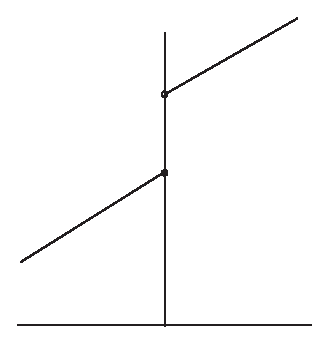
\includegraphics{PS/linear.eps}
  \caption{A piecewise linear function}
  \label{fig:discontinuous}
\end{figure}



We break the interval in two at $x=0$, forming two compact
intervals $[-1,0]$ and $[0,1]$.  We have continuous functions
$f_-:[-1,0]\to \R$ and $f_+:[0,1]$, such that
    $$
    f(x)=
    \begin{cases}
        f_-(x) & x\in[-1,0],\\
        f_+(x) & \text{otherwise}.
    \end{cases}
    $$
We have replaced the discontinuous function by a pair of
continuous functions on smaller intervals, at the expense of
duplicating the point of discontinuity $x=0$.  We view this pair
of functions as a single function $F$ on the compact topological
space with two components
    $$[-1,0]\times\{-\} \text{\ and\ } [0,1]\times\{+\}.$$
where $F(x,a) = f_a(x)$, and $a\in\{-,+\}$.

This is the approach that we follow in general with the Kepler
conjecture.  The function $\sigma$ is defined by a series of case
statements, and the function does not extend continuously across the
boundary of the cases.  However, in the degenerate cases that land
precisely between two or more cases, we form multiple copies of
decomposition star for each case, and place each case into a
separate compact domain on which the function $\sigma$ is
continuous.

This can be formalized as a {\it colored space}.  A colored space
is a topological space $X$ together with an equivalence relation
on $X$ with the property that no point $x$ is equivalent to any
other point in the same connected component as $x$.   We refer to
the connected components as colors, and call the points of $X$
{\it colored points}.  We call the set of equivalence classes of
$X$ the underlying uncolored space of $X$. Two colored points are
equal as uncolored points if they are equivalent under the
equivalence relation.
\index{colored!space}
\index{colored!points}

In our example, there are two colors ``$-$'' and ``$+$.''  The
equivalence class of $(x,a)$ is the set of pairs $(x,b)$ with the
same first coordinate.  Thus, if $x\ne0$, the equivalence class
contains one element $(x,\sign(x))$, and in the boundary case
$x=0$ there are two equivalent elements $(0,-)$ and $(0,+)$.

In our treatment of decomposition stars, there are various cases:
whether an edge has length less than or greater than $2t_0$, less
than or greater than $\sqrt8$, whether a face has circumradius
less than or greater than $\sqrt2$, and so forth. By duplicating
the degenerate cases (say an edge of exact length $2t_0$),
creating a separate connected component for each case, and
expressing the optimization problem on a colored space, we obtain
a continuous function $\sigma$ on a compact domain $X$.

The colorings have in general been suppressed in places from the
notation. To obtain consistent results, a statement about
$x\in[2,2t_0]$ should be interpreted as having an implicit
condition saying that $x$ has the coloring induced from the
coloring on the component containing $[2,2t_0]$.  A later
statement about $y\in[2t_0,\sqrt8]$ deals with $y$ of a different
color, and no relation between $x$ and $y$ of different colors is
assumed at the endpoint $2t_0$.




\shortversion{\chapter{Scoring~[Ferguson,~Hales]\index{Ferguson}}}
\longversion{\chapter{Scoring~[Ferguson,~Hales]\index{Ferguson}}}

\label{sec:scoring}

This \chap\  is coauthored by
Samuel P. Ferguson\index{Ferguson} and Thomas C. Hales.

In earlier \chaps, we describe each packing of unit balls by its set
$\Lambda\subset \ring{R}^3$ of centers of the packing.  We showed
that we may assume that our packings are saturated in the sense that
there is no room for additional balls to be inserted into the
packing without overlap. Lemma~\ref{lemma:deltabound} shows that the
Kepler conjecture follows if for each saturated packing $\Lambda$ we
can find a function $A:\Lambda\to\ring{R}$ with two properties: the
function is fcc-compatible and it is saturated in the sense of
Definition~\ref{def:negligible}.

The purpose of the first part of this \chap\ is to define a
function $A:\Lambda\to\ring{R}$ for every saturated packing
$\Lambda$ and to show that it is negligible.  The formula defining
$A$ consists of a term that is a correction between the volume of
the Voronoi cell $\Omega(v)$ and that of the $V$-cell $\op{VC}(v)$
and a further term coming from simplices of the $Q$-system that
have a vertex at $v$.

A major theorem in this \paper\ will be that this negligible
function is fcc-compatible.  The proof of fcc-compatibility can be
expressed as a difficult nonlinear optimization problem over the
compact topological space $\op{DS}$ that was introduced in
\Chap~\ref{sec:compact}.  In fact, we construct a continuous
function $A_0$ on the space $\op{DS}$ such that for each saturated
packing $\Lambda$ and each $v\in\Lambda$, the value of the function
$A$ at $v$ is a value in the range of the function $A_0$ on
$\op{DS}$. In this way, we are able to translate the
fcc-compatibility of $A$ into an extremal property of the function
$A_0$ on the space $\op{DS}$.

The proof of fcc-compatibility is more conveniently couched as an
optimization problem over a function that is related to the
function $A_0$ by an affine rescaling.   This new function is
called the score and is denoted $\sigma$.  (The exact relationship
between $A_0$ and $\sigma$ appears in Definition~\ref{def:score}.)
The function $\sigma$ is a continuous function on the space
$\op{DS}$. This function is defined in the final paragraphs of this
\chap.


\section{Definitions}
\label{sec:rules}


For every saturated packing $\Lambda$, and $v\in \Lambda$, there
is a canonically associated decomposition star $D(v,\Lambda)$. The
negligible function $A:\Lambda\to\ring{R}$ that we define is a
composite
  \begin{equation}
  A = A_0\circ D(\cdot,\Lambda)
  :\Lambda\to DS\to \ring{R},\quad v\mapsto D(v,\Lambda)\mapsto
  A_0(D(v,\Lambda)),
  \label{eqn:A}
  \end{equation}
where $A_0:\op{DS}\to\ring{R}$ is defined by
Equations~\ref{eqn:A1} and \ref{eqn:a1-sigma} below.  Each simplex
in the $Q$-system with a vertex at $v$ defines by translation to
the origin a simplex in the $Q$-system with a vertex at $0$
attached to $D(v,\Lambda)$. Let $\CalQ_0(D)$ be this set of
translated simplices at the origin. This set is determined by $D$.

\begin{definition} \label{def:context}
Let $Q$ be a quarter in $\CalQ_0(D)$.  We say that the {\it
context\/} of $Q$ is $\x(p,q)$ if there are $p$ anchors and $p-q$
quarters along the diagonal of $Q$. Write $c(Q,D)$ for the context
of $Q\in\CalQ_0(D)$.
\end{definition}\index{context (of a quarter)}

$q$ is the number of ``gaps'' between anchors around the diagonal.
For example, the context of a quarter in a quartered octahedron is
$\x(4,0)$.  The context of a single quarter is $\x(2,1)$.
%The
%only possible contexts of upright quarters in a quad cluster are
%$\x(4,0)$, $\x(3,1)$, and $\x(2,1)$. Of course, $Q$ and $\hat Q$
%have the same context. The definition of $\sigma(Q)$ depends on
%the context of $Q$.


The function $A_0$ will be defined to be
a continuous function on $\op{DS}$ of the
form
  \begin{equation}
  A_0(D) = -\op{vol}\,(\Omega(D)) + \op{vol}\,(\op{VC}(D)) +
   \sum_{Q\in\CalQ_0(D)} A_1(Q,c(Q,D),0).
   \label{eqn:A1}
   \end{equation}
Thus, the function $A_0$ measures the difference in volume between
the Voronoi cell and $V$-cell, as well as certain contributions
$A_1$ from the $Q$-system. The function $A_1(Q,c,v)$ depends on
$Q$, its context $c$, and a vertex $v$ of $Q$.  The function
$A_1(Q,c,v)$ will not depend on the second argument when $Q$ is a
quasi-regular tetrahedron.  (The context is not defined for such
simplices.)



\begin{definition} \label{def:rogers}
An {\it orthosimplex} consists of the convex hull of
$\{0,v_1,v_1+v_2,v_1+v_2+v_3\}$, where $v_2$ is a vector
orthogonal to $v_1$, and $v_3$ is orthogonal to both $v_1$ and
$v_2$.  We can specify an orthosimplex up to congruence by the
parameters $a = |v_1|$, $b=|v_1+v_2|$, and $c=|v_1+v_2+v_3|$,
where $a\le b\le c$. This parametrization of the orthosimplex
departs from the usual parametrization by the lengths $|v_1|$,
$|v_2|$, $|v_3|$. For $a\le b\le c$,  the {\it Rogers simplex\/}
$R(a,b,c)$ is an orthosimplex of the form
$$R(a,b,c)=S(a,b,c,\sqrt{c^2-b^2},\sqrt{c^2-a^2},\sqrt{b^2-a^2}).$$
See Figure~\ref{fig:rogers}.
%
 \index{Rogers simplex}
 \index{orthosimplex}
\end{definition}

\begin{figure}[htb]
  \centering
  \includegraphics{PS/rogers.eps}
  \caption{The Rogers simplex is an orthosimplex.}
  \label{fig:rogers}
\end{figure}

\begin{definition}\label{def:quoin}\index{quoin}
Let $R$ be a Rogers simplex.  We define the {\it quoin} of $R$ to
be the  wedge-like solid (a quoin) situated above $R$. It is
defined as the solid bounded by the four planes through the faces
of $R$ and a sphere of radius $c$ at the origin. (See
Figure~\ref{fig:quoin}.)   We let $\quo(R)$ be the volume of the
quoin over $R$.  \shortversion{An explicit formula appears in
\cite{KC}.}  \longversion{If $R=R(a,b,c)$ is a Rogers simplex, the
volume $\quo(R)$ is given explicitly as follows\index{Rogers
simplex}
    \begin{equation}
    \begin{array}{lll}
    6\quo(R) &= (a+2c)  %
    % -(a^2+ac-2c^2)
    (c-a)^2\arctan(e)
        +a(b^2-a^2)e\\&-4c^3\arctan(e(b-a)/(b+c)),
    \label{eqn:3.3}
    \end{array}
    \end{equation}
where $e\ge0$ is given by $e^2(b^2-a^2)=(c^2-b^2)$.}
%
 \index{quoin}
\end{definition}


\begin{figure}[htb]
  \centering
  \includegraphics{PS/quoin.eps}
  \caption{The quoin above a Rogers simplex is the part of the
  shaded solid outside
   the illustrated box.  It is bounded by the shaded planes, the plane through
   the front face of the box, and a sphere
   centered at the origin passing through the opposite corner of the box.}
  \label{fig:quoin}
\end{figure}

Let $S$ be a simplex and let $v$ be a vertex of that simplex. Let
$\op{VC}(S,v)$ be the subset of $|S|$ consisting of points closer
to $v$ than to any other vertex of $S$. By
Lemma~\ref{lemma:Q-divide}, if $S\in\CalQ_0(D)$, then
$$\op{VC}(S,0) = \op{VC}(D)\cap |S|.$$
Under the assumption that $S$ contains its circumcenter and that
every one of its faces contains its circumcenter, an explicit
formula for the volume $\op{vol}(\op{VC}(S,v))$ has been
calculated in \cite[Section~8.6.3]{part1}. This volume formula is
an algebraic function of the edge lengths of $S$, and may be
analytically continued to give a function of $S$ with chosen
vertex $v$:
  $$\op{vol}\,\op{VC}^\op{an}(S,v).$$

\begin{lemma}\label{lemma:cap-rogers}
Let $B(0,t)$ be a ball of radius $t$ centered at the origin.  Let
$v_1$ and $v_2$ be vertices.  Assume that $|v_1|< 2t$ and $|v_2|<2
t$.  Truncate the ball by cutting away the caps
   $$\op{cap}_i = \{x\in B(0,t) :  |x- v_i| < |x|\}.$$
Assume that the circumradius of the triangle $\{0,v_1,v_2\}$ is
less than $t$. Then the intersection of the caps $\op{cap}_1\cap
\op{cap}_2$ is the union of four quoins.
\end{lemma}

\begin{proof} This is true by inspection.  See Figure~\ref{fig:capriquoin}.
Slice the intersection $\op{cap}_1\cap\op{cap}_2$ into four pieces
by two perpendicular planes: the plane through $\{0,v_1,v_2\}$,
and the plane perpendicular to the first and passing through $0$
and the circumcenter of $\{0,v_1,v_2\}$.  Each of the four pieces
is a quoin.
\end{proof}

\begin{figure}[htb]
  \centering
  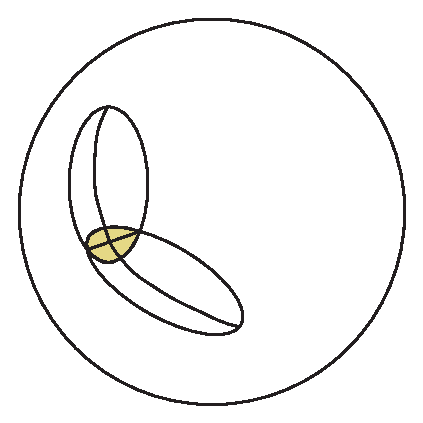
\includegraphics{PS/capriquoin.eps}
  \caption{The intersection of two caps on the unit ball can
   be partitioned into four quoins (shaded).}
  \label{fig:capriquoin}
\end{figure}

\begin{definition}\label{def:sol}
Let $v\in\ring{R}^3$ and let $X$ be a measurable subset of
$\ring{R}^3$. Let $\sol(X,v)$ be the area of the radial projection
of $X\setminus\{0\}$ to the unit sphere centered at the origin. We
call this area the {\it solid angle\/} of $X$ (at $v$).  When
$v=0$, we write the function as $\sol(X)$.
 %
 \index{sol}
 \index{solid angle}
\end{definition}


Let $S=\{v_0,v_1,v_2,v_3\}$ be a simplex. Fix $t$ in the range
$t_0\le t\le\sqrt2$.  Assume that $t$ is at most the circumradius
of $S$. Assume that it is at least the circumradius of each of the
faces of $S$.  Let $\op{VC}_t(S,v_0)$ be the intersection of
$\op{VC}(S,v_0)$ with the ball $B(v_0,t)$. Under the assumption
that $S$ contains its circumcenter and that every one of its faces
contains it circumcenter, an explicit formula for the volume
$$\op{vol}(\op{VC}_t(S,v_0))$$ is calculated by means of
Lemma~\ref{lemma:cap-rogers} through a process of inclusion and
exclusion. In detail, start with $|S|\cap B(v_0,t)$. Truncate this
solid by caps $\op{cap}_1$, $\op{cap}_2$,\index{cap} and
$\op{cap}_3$ bounded by the sphere of radius $t$ centered at $v_0$
and the perpendicular bisectors (respectively) of $\{v_0,v_1\}$,
$\{v_0,v_1\}$, $\{v_0,v_2\}$.  If we subtract the volume of each
cap $\op{cap}_i$, then we must add back the volume of the doubly
counted intersections of the caps.  The intersections of caps are
given as quoins (Lemma~\ref{lemma:cap-rogers}).  This leads to the
following formula. Let $h_i = |v_i|/2$ and
$\eta_{ij}=\eta(0,v_i,v_j)$, and let $S_3$ be the group of
permutations of $\{1,2,3\}$ in
\begin{equation}
   \op{vol}\,\op{VC}_t(S,v_0) =
   \sol(S)/3 - \sum_{i=1}^3 \frac{\dih(S,v_i)}{2\pi}\op{vol}\,\op{cap_i}
   +\sum_{(i,j,k)\in S_3} \quo(R(h_i,\eta_{ij},t)).
   \label{eqn:vol-theta-0}
\end{equation}


We extend Formula~\ref{eqn:vol-theta-0} by setting
    $$\quo(R(a,b,c)) = 0,$$
if the constraint $a < b < c$ fails to hold.  Similarly, set
$\op{vol}\,\op{cap}_i=0$ if $|v_i|\ge 2t$.  With these
conventions,  Formula~\ref{eqn:vol-theta-0} extends to all
simplices.  We write the extension of $\op{vol}\,\op{VC}_t(S,v)$
as
$$\op{vol}\,{\op{VC}^+_t}(S,v).$$



\begin{definition}\label{def:svor}
   Let\footnote{In the paper \cite{spp}, the volumes in this definition were
   volumes of Voronoi cells, and hence the notation $\vor$ for the function was
adopted. We retain $\vor$ in the notation, although this direct
connection with Voronoi cells has been lost.}
      $$
      \svor(S,v) = 4(-\doct \op{vol}\,\op{VC}^{\op{an}}(S,v)
         +\sol(S,v)/3),$$
      $$
      \svor(S,v,t) = 4(-\doct \op{vol}\,\op{VC}^+_{t}(S,v)
         +\sol(S,v)/3),$$
   and
      $$
      \svor_0(S,v) = \svor(S,v,t_0).
      $$
   When it is clear from the context that the vertex $v$ is
   fixed at the origin, we drop $v$ from the notation of these
   functions.
   If $S=\{v_1,v_2,v_3,v_4\}$, we define $\Gamma(S)$ as the average
   \begin{equation}
   \Gamma(S) = \frac{1}{4}\sum_{i=1}^4\svor(S,v_i).
   \label{eqn:gamma}
   \end{equation}
   The average $\Gamma(S)$ is called the {\it compression} of $S$.
%
 \index{compression}
 \index{ZZcamma@$\Gamma$}
\end{definition}

\begin{definition}
Let $Q$ be a quarter.   Let $\eta^+(Q)$ be the maximum of the
circumradii of the two faces of $Q$ along the diagonal of $Q$.
\end{definition}

Let $Q$ be a simplex in the $Q$-system.  We define an involution
$v\to \hat v$ on the vertices of $Q$ as follows.  If $Q$ is a
quarter and $v$ is an endpoint of the diagonal, then let $\hat v$
be the opposite endpoint of the diagonal.  In all other cases, set
$\hat v = v$.

We are ready to complete the definition of the function
$A:\Lambda\to\ring{R}$.  The definition of $A$ was reduced to that
of $A_0$ in Equation~\ref{eqn:A}.  The function $A_0$ was reduced
in turn to that of $A_1$ in Equation~\ref{eqn:A1}. To complete the
definition, we define $A_1$.

\begin{definition}\label{def:sigma}
Set
   \begin{equation}\label{eqn:a1-sigma}
   A_1(S,c,v) = -\op{vol}\,\op{VC}(S,v)+
      \frac{\sol(S,v)}{3\doct} - \frac{\sigma(S,c,v)}{4\doct}.
      \end{equation}  where $\sigma$ is given as follows:
      %
      \index{AZ1@$A_1$}
      \index{ZZsigma@$\sigma$}
\begin{enumerate}
\item If $S$ is a quasi-regular tetrahedron:
   \begin{enumerate}
      \item If the circumradius of $S$ less than $1.41$, set
         $$\sigma(S,-,v)=\Gamma(S)$$
      \item If the circumradius of $S$ is at least $1.41$, set
         $$\sigma(S,-,v)=\svor(S,v).$$
   \end{enumerate}
\item If $S$ is a strict quarter:
   \begin{enumerate}
      \item If $\eta^+(S) <\sqrt2$:
         \begin{enumerate}
         \item If the context $c$ is $(2,1)$ or $(4,0)$, set
                  $$\sigma(S,c,v)=\Gamma(S)$$
         \item If the context of $S$ is anything else, set
                  $$\sigma(S,c,v)=\Gamma(S) +
                     \frac{\svor_0(S,v)-\svor_0(S,\hat v)}{2}.$$
         \end{enumerate}
      \item If $\eta^+(S) \ge\sqrt2$:
         \begin{enumerate}
         \item If the context of $S$ is $(2,1)$, set
                  $$\sigma(S,c,v)=\svor(S,v).$$
         \item If the context of $S$ is $(4,0)$, set
                  $$\sigma(S,c,v)=\frac{\svor(S,v)+\svor(S,\hat v)}{2}.$$
         \item If the context of $S$ is anything else, set
                  $$\sigma(S,c,v)=\frac{\svor(S,v)+\svor(S,\hat
                  v)}{2}
                     +\frac{\svor_0(S,v)-\svor_0(S,\hat v)}{2}.$$
         \end{enumerate}
   \end{enumerate}
\end{enumerate}
When the context and vertex $v$ are given, we often write
$\sigma(S)$ or $\sigma(S,v)$ for $\sigma(S,c,v)$.

When $\eta^+<\sqrt2$, we say that the quarter has compression type.
Otherwise, we say it has Voronoi type.  To say that a quarter has
compression type means that $\Gamma(S)$ is one term of the function
$\sigma(S,v)$. It does not mean that $\Gamma(S)$ is equal to
$\sigma(S,v)$.
%
 \index{Voronoi type}
 \index{compression type}
\end{definition}

\longversion{The definition of $\sigma$ on quarters can be expressed
a second way in terms of a function $\mu$.  If $S$ is a quarter, set
    \begin{equation}
    \mu(S,v)=\begin{cases}
    \Gamma(S),&  \text{ if }\eta^+(S)<\sqr2,\\
    \svor(S,v),& \hbox{otherwise.}\end{cases}
    \label{eqn:3.8}
    \end{equation}
If $S$ is a flat quarter, we have $\sigma(S,c,v)=\mu(S,v)$, for all
contexts $c$.}

\longversion{Suppose $S$ is an upright
quarter.\index{quarter!upright} Definition~\ref{def:sigma} can be
expressed as follows.}

\longversion{
\begin{itemize}
 \item context $\x(2,1)$:  Set $\sigma(S,c,v)=\mu(S,v)$.
 \item context
    $\x(4,0)$:  Set $\sigma(S,c,v)=(\mu(S,v)+\mu(S,\hat v))/2$.
 \item other contexts:
 Set $\sigma(S,c,v)=(\mu(S,v)+\mu(S,\hat v)+ \svor_0(S,v) - \svor_0(S,\hat v))/2$.
\end{itemize}
 }


\begin{lemma}  $A_0:\op{DS}\to\ring{R}$ is continuous.
\end{lemma}

\begin{proof}
The continuity of $D\mapsto\op{vol}\,\op{VC}(D)$ is proved in
Lemma~\ref{lemma:vc-cont}.  The continuity of
$D\mapsto\op{vol}\,\Omega(D)$ is similarly proved.  The terms
$\op{vol}\,\op{VC}(S,v)$ and $\sol(S,v)$ are continuous. To complete
the proof we check that the function $\sigma(S,c,v)$ is continuous.
It is not continuous when viewed as a function of the set of
quarters, because of the various cases breaking at circumradius
$1.41$ and $\eta^+(S)=\sqrt2$.  However, these cutoffs have been
inserted into the data defining a decomposition star (in the
indexing sets $I_8$ and $I_9$).  Thus, the different cases in the
definition of $\sigma(S,c,v)$ land in different connected components
of the space $\op{DS}$ and continuity is obtained.
\end{proof}

We conclude this section with a result that will be of use in the
next section.

\begin{lemma}\label{lemma:A1-cancel}
Let $S=\{v_1,v_2,v_3,v_4\}$ be a simplex in the $S$-system,  and $c$
its context.   Then
   $$\sum_{i=1}^4 A_1(S,c,v_i)=0.$$
\end{lemma}

\begin{proof}
   By Formula~\ref{eqn:a1-sigma}, this is equivalent to
      \begin{equation}
      \sum_{i=1}^4 \sigma(S,c,v_i) = \sum_{i=1}^4
      \svor(S,c,v_i).
      \label{eqn:sigma-4}
      \end{equation}
Equation~\ref{eqn:sigma-4} is evident from
Definition~\ref{def:sigma} for $\sigma$.  In fact, the terms of the
form $\svor_0$ have opposing signs and cancel when we sum. The other
terms are weighted averages of the terms $\svor(S,c,v_i)$.
Equation~\ref{eqn:sigma-4} is thus established by noting that a sum
is unaffected by taking weighted averages of its terms.
\end{proof}


\section{Negligibility} \label{sec:negligible}

Let $B(x,r)$ be the closed ball of radius $r\in\ring{R}$ centered
at $x$.  Let $\Lambda(x,r)=\Lambda\cap B(x,r)$.

Recall from Definition~\ref{def:negligible} that a function
$A:\Lambda\to\ring{R}$ is said to be {\it negligible} if there is
a constant $C_1$ such that for all $r\ge1$, we have
   $$\sum_{v\in\Lambda(x,r) } A(v) \le C_1 r^2.$$
%
 \index{negligible}


Recall that a function $A: \Lambda\to\ring{R}$ given by
Equation~\ref{eqn:A}.  Explicitly, let
   $$A(v) = A_0(D(v,\Lambda)),$$
where $A_0$ in turn depends on functions $A_1$ and $\sigma$, as
determined by Equations~\ref{eqn:A1} and \ref{eqn:a1-sigma}, and
Definition~\ref{def:sigma}.

\begin{theorem}\label{lemma:negligible}
The function $A$ of Equation~\ref{eqn:A} is negligible.
\end{theorem}

\begin{proof} First we consider a simplification, where we replace
   $A$ with $A'$ defined by
      $$
      A'(v,\Lambda) = -\op{vol}(\Omega(D(v,\Lambda)))+
         \op{vol}(\op{VC}(D(v,\Lambda))).$$
(That is, at first we ignore the function $A_1$.) The Voronoi
cells partition $\ring{R}^3$, as do the $V$-cells.  We have
$\Omega(v,\Lambda)\subset B(v,2)$ (by saturation) and
$\op{VC}(v,\Lambda)\subset B(v,2\sqrt3)$ (by
Definition~\ref{def:phi}). Hence the Voronoi cells with $v\in
\Lambda(x,r)$ cover $B(x,r-2)$. Moreover, the $V$-cells with $v\in
\Lambda(x,r)$ are contained in $B(x,r+2\sqrt3)$.  Hence
   $$
   \sum_{v\in\Lambda(x,r)} A'(v) \le -\op{vol}\,B(x,r-2)
      +\op{vol}\,B(x,r+2\sqrt3)\le C_1' r^2
   $$
for some constant $C_1'$.

If we do not make the simplification, we must also include the sum
   $$\sum_{v\in\Lambda(x,r)} \sum_{Q\in\CalQ_v(D(v,\Lambda))}
      A_1 (Q,c,v).$$
Each quarter $Q=\{v_1,v_2,v_3,v_4\}$ in the $Q$-system occurs in
four sets $\CalQ_{v_i}(D(v_i,\Lambda))$.  By
Lemma~\ref{lemma:A1-cancel} the sum cancels, except when some
vertex of $Q$ lies inside $\Lambda(x,r)$ and another lies outside.
Each such simplex lies inside a shell of width $2\sqrt8$ around
the boundary.  The contribution of such boundary terms is again
bounded by a constant times $r^2$.  This completes the proof.
\end{proof}


\section{Fcc-compatibility}

We have constructed a negligible function $A$.  The rest of this
\paper\ will prove that this function is fcc-compatible.   This
section translates fcc-compatibility into a property that will be
easier to prove.  To begin with, we introduce a rescaled version
of the function $A$.

\begin{definition}\label{def:score}
Let $\sigma:\op{DS}\to\ring{R}$ be given by
   $$\sigma(D) = -4\doct (\op{vol}\,\Omega(D) + A_0(D)) +
   16\pi/3.$$
It is called the {\it score} of the decomposition star.
%
 \index{score}
 \index{ZZsigma@$\sigma(D)$}
\end{definition}

Recall from Definition~\ref{def:pt} the constant $\pt\approx
0.05537$.  This constant is called a point.\index{point}

\begin{lemma}\label{lemma:8pt-compat}
Let $A_0$, $A$, and $\sigma$ be the functions defined by
Equations~\ref{eqn:A}, \ref{eqn:A1}  \ref{eqn:a1-sigma}, and
Definition~\ref{def:sigma}. The following are equivalent.
\begin{enumerate}
  \item The minimum of the function on $\op{DS}$ given by
      $$D\mapsto \op{vol}\,\Omega(D) + A_0(D)$$
is $\sqrt{32}$.
  \item The maximum of $\sigma$ on $\op{DS}$ is $8\,\pt$.
\end{enumerate}
Moreover, these statements imply
\begin{itemize}
  \item For every saturated packing $\Lambda$,
  the function $A$ is
  fcc-compatible.
\end{itemize}
\end{lemma}

(Eventually, we prove fcc-compatibility by proving
$\sigma(D)\le8\,\pt$ for all $D\in\op{DS}$.)

\begin{proof} To see the equivalence of the first and second statements,
use Definition~\ref{def:score},  and the identity
   $$8\,\pt = -4\doct (\sqrt{32}) + 16 \pi/3.$$
(Note that this identity is parallel in form with
Definition~\ref{def:score} for $\sigma$.)

For a given saturated packing $\Lambda$, the function $A$ has the
form $A(v) = A_0(D(v,\Lambda))$.  Also, $\Omega(D(v,\Lambda))$ is
a translate of $\Omega(v)$, the Voronoi cell at $v$.  In
particular, they have the same volume.  Thus,
$\op{vol}\,\Omega(v)+A(v)$ lies in the range of the function
   $$\op{vol}\,\Omega(D) + A_0(D)$$
on $\op{DS}$.  The minimum of this function is $\sqrt{32}$ by the
first of the equivalent statements.  It now follows from the
definition of fcc-compatibility, that $A:\Lambda\to\ring{R}$ is
indeed fcc-compatible.
\end{proof}

\begin{theorem}\label{lemma:exista}
If the maximum of the function $\sigma$ on
$\op{DS}$ is $8\,\pt$, then for every saturated packing $\Lambda$
there exists a negligible fcc-compatible function $A$.
\end{theorem}

\begin{proof} This follows immediately from Theorem~\ref{lemma:negligible}
and Lemma~\ref{lemma:8pt-compat}.
\end{proof}



\section{Scores of Standard Clusters}
\label{sec:ssc}

The last section introduced a function $\sigma$ called the score. We
show that the function $\sigma$ can be expressed as a sum over terms
attached to each of the standard regions.

\begin{definition} \label{def:standard-cluster}
A {\it standard cluster\/} is a pair $(R,D)$ where $D$ is a
decomposition star and $R$ is one of its standard regions.  A {\it
quad cluster\/} is the standard cluster obtained when the standard
region is a quadrilateral.
\end{definition}
%
 \index{cluster!standard}
 \index{cluster!quad}
 \index{quad cluster}

%Recall $|S|$ is the convex hull of a set $S\subset
%\ring{R}^3$.

We break $\sigma$ into a sum
   \begin{equation}
   \sigma(D) = \sum_R\,\sigma_R(D),
   \end{equation}
indexed by the standard clusters $(R,D)$.  Let
   $$
   \op{VC}_R(D) = \op{VC}(D)\cap \op{cone}(R),
   $$
whenever $R$ is a measurable subset of the unit sphere.  Let
   $$
   \CalQ_0(R,D) = \{Q\in \CalQ_0(D) : Q\subset \op{cone}(R)\}.
   $$
By Lemma~\ref{lemma:Q-in-region},
 each $Q$ is entirely contained in the cone over a single
standard region.

\begin{definition} \label{def:score-std-region}
   Let $R$ be a measurable subset of the unit sphere.  Set
      $$
      \vor_R(D) =4\left(-\doct \op{vol}\,\op{VC}_R(D)  + \sol(R)/3\right)
      $$
      Let $R$ be a standard region. Set
      $$
      \sigma_R(D) = \vor_R(D) - 4\doct
         \sum_{Q\in\CalQ_0(R,D)} A_1(Q,c(Q,D),0).
      $$
\index{vzorR@$\vor_R$} \index{zzsigmaR@$\sigma_R$}
\end{definition}

\begin{lemma} $\sigma(D) = \sum_R\sigma_R(D)$, where the sum runs
over all standard regions $R$.
\end{lemma}

\begin{proof}
   $$
   \begin{array}{lll}
      \sigma(D)
      &= -4\doct (\op{vol}\,\Omega(D) + A_0(D))+16\pi/3\\
      &= -4\doct (\op{vol}\,\op{VC}(D)+\sum_{Q\in\CalQ_0(D)}
         A_1(Q,c(Q,D),0)) + (4) (4\pi/3)\\
      &= \sum_R 4\left (-\doct \op{vol}\,\op{VC}_R(D) -\doct
         \sum_{Q\in\CalQ_0(R,D)} A_1(Q,c(Q,D),0) +
         \sol(R)/3\right).
   \end{array}
   $$
\end{proof}

\longversion{
Also, we have
    \begin{equation}
    \op{vor}(D)=\sum_{R\in \CalR(D)}
    \op{vor}_R(D).
    \label{eqn:vorD}
    \end{equation}
    }

\begin{lemma}\label{lemma:R'}
Let $R'\subset R$ be the part of a standard region that does not
lie in any cone over any $Q\in Q_0(R,D)$.  Then
   $$
   \sigma_R(D) = \vor_{R'}(D)
      + \sum_{Q\in\CalQ_0(R,D)} \sigma(Q,c(Q,D),0).
   $$
\end{lemma}

\begin{proof} Substitute the definition of $A_1$
(Equation~\ref{eqn:a1-sigma}) into the definition of
$\sigma_R(D)$, noting that $\op{VC}(Q,0) = \op{VC}_{R''}(D)$,
where $R''$ is the intersection of $Q$ with the unit sphere.
\end{proof}

\begin{remark}   Lemma~\ref{lemma:R'} explains why we have chosen
the same symbol $\sigma$ for the functions $\sigma_R(D)$ and
$\sigma(Q,c,v)$.  We can view Lemma~\ref{lemma:R'} as asserting a
linear relation in the functions $\sigma$:
   $$\sigma_R(D) = \sigma_{R'}(D) + \sum \sigma(Q,c,0).$$
The sum runs over $Q\in\CalQ_0$ that lie in the cone over $R$.
\end{remark}

\longversion{\section{Scores of Simplices and Cones}}

\longversion{Many of the functions in this paper are defined by
terms involving volumes of simple solids.  To give estimates on the
functions, it is often convenient to partition the solids into
smaller pieces and then define corresponding functions on each of
the pieces.  For this reason, we define some variants of the
functions $\vor$ and $\sigma$.}

\longversion{
\begin{remark}\label{remark:vor}\index{vor}\index{c-vor}\index{score}
We now define a few more variants of the function $\vor$. The
function $\svor$ and its truncated version  $\svor(\cdot,t)$ have
been defined already. The function $\vor_R(D)$ will also be given a
truncated version $\vor_R(D,t)$, for a real truncation parameter
$t\ge 0$. The special case, $\vor_R(D,t_0)$ will be abbreviated
$\vor_{0,R}(D)$. There will be another variant $\op{r-vor}$ for
Rogers simplices, and another $\op{c-vor}$ for general sets.  The
general form of these functions is
    $$\op{c-vor}(X) = 4 (-\doct\op{vol}(X) + \sol(X)/3),$$
for any subset $X\subset \ring{R}^3$.   The differences between the
different versions of $\vor$ come from the different choices of the
set $X$ and the way they are parameterized.
\end{remark}}

\longversion{
\begin{definition}  \label{def:r-vor}\index{r-vor}
Let $R=R(a,b,c)$ be a Rogers simplex. Assume that the
vertex terminating the edges of lengths $a$, $b$, and $c$ is
situated at the origin. Let
    $$\op{r-vor}(R) = 4 (-\doct\op{vol}(R) + \sol(R)/3).$$
\end{definition}}


% \index{Voronoi function} We define the simplex
%version $\svor$ of the function as follows. We begin with its
%definition for simplices $S$ whose faces have positive
%orientation. Assume that $S$ has a distinguished vertex $v$, which
%e fix at the origin. Let $\sol(S)$ be the solid angle of $S$ at
%its distinguished vertex.\index{sol} Set
%$\doct=(\pi-4\arctan(\sqr2/5))/\sqr8$. Set
%    \begin{equation}
%   \svor(S) = 4(-\doct \op{vol}(\op{VC}(S,0)) + \sol(S)/3),
%   \label{eqn:3.1}
%    \end{equation}
%This formula may be analytically continued to simplices $S$ with
%negatively oriented faces, and $\svor(S)$ is defined in general by
%this analytic continuation. A formula for $\svor$ is found in
%\cite[Sec. 8.6]{part1}.  Let $S_1,\ldots, S_4$ be equal to $S$
%as unlabeled simplices, but with different distinguished vertices.

\longversion{
\begin{definition}\label{def:cone}
 Let $C(h,t)$ denote the compact cone of height $h$
and circular base. Set
%of area $\pi(t^2-h^2)$. Set
    $$
    \phi(h,t)=2(2-\doct  t h (h+t))/3.
    $$
\index{right circular cone}\index{cone}
 Then
    \begin{equation}
    \op{c-vor}(C(h,t))=2\pi(1-h/t)\phi(h,t).
    \label{eqn:3.2}
    \end{equation}
 \end{definition}
    }

\longversion{
\begin{remark}\label{remark:score}
Below, we introduce variants of the function $\sigma$. We have
already encountered $\sigma$ in Definitions~\ref{def:sigma},
\ref{def:score}, and \ref{def:score-std-region}. Informally, we call
$\sigma$ (and various functions that are closely related to it) the
{\it score}. Equation~\ref{eqn:3.2} represents the {\it score\/} of
$C(h,t)$. The solid angle of $C(h,t)$ is $2\pi(1-h/t)$, so
$\phi(h,t)$ is the score per unit area. Also, $\phi(t,t)$ is the
score per unit area of a ball of radius $t$. That is, $\phi(t,t) =
4(-\doct\op{vol}/\sol + 1/3)$.\index{score}
\end{remark}
}


\longversion{ We set
    \begin{equation}
    \begin{array}{lll}
    \svor(S,t) &=
    \sol(S)\phi(t,t)
    +\sum_{i=1,\ h_i\le t}^3 d_i (1-h_i/t) (\phi(h_i,t)-
    \phi(t,t)) \\
    &-\sum_{(i,j,k)\in S_3}
    4\doct
    \quo(R(h_i,\eta(y_i,y_j,y_{k+3}),t)).
    \label{eqn:3.5}
    \end{array}
    \end{equation}
In the definition, we adopt the convention that $\quo(R)=0$, if
$R=R(a,b,c)$ does not exist (that is, if the condition
    $0< a\le b\le c$
is violated). In the second sum, $S_3$ is the set of permutations on
three letters. This definition is compatible with
Definition~\ref{def:svor}.}


%This formula has a simple geometric interpretation when the
%circumradius of $S$ is greater than $t$ and the circumradius of
%each face is less than $t$. It represents the score\index{score}
%of the part of the Voronoi cell at the origin that lies inside $S$
%and inside a ball of radius $t$.  This can be seen geometrically
%from Figure~\ref{fig:diag36}, which depicts the intersection of
%$S$ with the Voronoi cell as three quadrilaterals forming a
%triangle. The truncation in the second frame is shown as a shaded
%region. The truncated volume can be decomposed into a solid angle
%term, three conic terms, and six quoins (with appropriate sign
%conventions).  Hence the formula for $\svor(S,t)$. }



\longversion{ Similarly, we define $\vor_P(D,t)$ for arbitrary
standard clusters $(P,D)$.  (We shift notation from $R$ to $P$ for a
standard region to avoid conflict with Rogers simplices $R$ in the
following definition.)  Extending the notation in an obvious way, we
have
    \begin{equation}
    \begin{array}{lll}
    \vor_P(D,t) &=
    \sol(P)\phi(t,t)
    +\sum_{|v_i|\le 2t} d_i (1-|v_i|/(2t)) (\phi(|v_i|/2,t)-
    \phi(t,t)) \\
    &-\sum_{R} 4\doct \quo(R).
    \label{eqn:3.7}
    \end{array}
    \end{equation}
The first sum runs over vertices in $P$ of height at most $2t$. The
second sum runs over Rogers simplices $R(|v_i|/2,\eta(F),t)$ in $P$,
where $F=\{0,v_1,v_2\}$ is a face of circumradius $\eta(F)$ at most
$t$, formed by vertices in $P$.  The constant $d_i$ is the total
dihedral angle along $\{0,v_i\}$ of the standard cluster. The
truncations $t=t_0=1.255$ and $t=\sqr2$ will be of particular
importance.
    Set $A(h) = (1-h/t_0) (\phi(h,t_0)-\phi(t_0,t_0))$.\index{A}}

\longversion{
\begin{remark}  We have introduced both untruncated and truncated
versions of functions $\vor$ and $\sigma$.  The truncated versions
are used to give upper bounds on the untruncated versions.  For
example,  in the function $\sigma(D)$, the $V$-cell contributes
through its volume, as in Remark~\ref{remark:vor}.  The volume
appears with a negative coefficient $-4\doct$.  Thus, we obtain an
upper bound on $\sigma(D)$ by discarding bits of volume from the
$V$-cell.   This suggests that we might try to give upper bounds on
the score $\sigma(D)$ by truncating the $V$-cell in various ways.
This is the reason for the truncated versions of these functions.
\end{remark}}

\longversion{\section{The Example of a Dodecahedron}}

\longversion{
\begin{example}  The following example illustrates why better bounds
on the density of packings can be obtained with $\sigma(D)$ than
with a naive approach based on the volume of Voronoi cells.  By
scoring quasi-regular tetrahedra with the compression function
$\Gamma(S)$ rather than $\op{s-vor}(S)$, we will find that the score
is lowered below $8\,\pt$ for configurations with many quasi-regular
tetrahedra. To work one example, let us assume that the
decomposition star consists of $12$ vertices located at distance $2$
from the origin, at the vertices of a regular icosahedron. The score
is approximately
   $$20\,\Gamma(S(2,2,2,2.1092,2.1092,2.1092) \approx 1.8\,\pt < 8\,\pt.$$
If $\op{s-vor}(S)$ had been used, the score would violate Theorem
1.7:
   $$20\,\op{s-vor}(S) \approx 13.5493\,\pt > 8\,\pt.$$
(This is tied to the fact that the regular dodecahedron of
inradius $1$ has smaller volume than the rhombic dodecahedron of
inradius $1$.)
\end{example}
}
